%
% PROJECT: <ETD> Electronic Thesis and Dissertation Initiative
%   TITLE: LaTeX report template for ETDs in LaTeX
%  AUTHOR: Neill Kipp, nkipp@vt.edu
%     URL: http://etd.vt.edu/latex/
% SAVE AS: etd.tex
% REVISED: September 6, 1997 [GMc 8/30/10]
% 

% Instructions: Remove the data from this document and replace it with your own,
% keeping the style and formatting information intact.  More instructions
% appear on the Web site listed above.

\documentclass[12pt]{report}
\usepackage{cite}
\usepackage{amsmath,amssymb}
\usepackage{framed}
\usepackage{todonotes}
\usepackage{graphicx}
\usepackage{color}
\graphicspath{ {images/} }
\usepackage{float}
\usepackage{epsfig}
\usepackage{subfigure}
\usepackage{url}
\usepackage{comment}
\usepackage{color}
\usepackage[linesnumbered,lined,boxed,commentsnumbered]{algorithm2e}
\usepackage{physics}

\newtheorem{mydef}{Definition}
\newcommand{\pcomment}[1]{{\color{red}{#1}}}
\newcommand{\eg}{\textit{e.g.}}
\newcommand{\ie}{\textit{i.e.}}
\usepackage[acronym]{glossaries}
\setlength{\textwidth}{6.5in}
\setlength{\textheight}{8.5in}
\setlength{\evensidemargin}{0in}
\setlength{\oddsidemargin}{0in}
\setlength{\topmargin}{0in}

\setlength{\parindent}{0pt}
\setlength{\parskip}{0.1in}

% Uncomment for double-spaced document.
%\renewcommand{\baselinestretch}{2}
\newacronym{uav}{UAV}{Unmanned Aerial Vehicle}
\newacronym{gps}{GPS}{Global Positioning System}

\makeglossaries
% \usepackage{eps

\begin{document}

\thispagestyle{empty}
\pagenumbering{roman}
\begin{center}

% TITLE
{\Large 
Reinforcement Learning with Gaussian Processes for Unmanned Aerial Vehicle Navigation
}

\vfill

Nahush Gondhalekar

\vfill

Thesis submitted to the Faculty of the \\
Virginia Polytechnic Institute and State University \\
in partial fulfillment of the requirements for the degree of

\vfill

Master Of Science \\
in \\
Computer Engineering

\vfill

Pratap Tokekar, Chair \\
Haibo Zeng \\
A. Lynn Abbott

\vfill

June 23, 2017 \\
Blacksburg, Virginia

\vfill

Keywords: Reinforcement Learning,Gaussian Processes 
\\
Copyright 2017, Nahush Gondhalekar

\end{center}

\pagebreak

\thispagestyle{empty}
\begin{center}

{\large Reinforcement Learning with Gaussian Processes for Unmanned Aerial Vehicle Navigation}

\vfill

Nahush Gondhalekar

\vfill

(ABSTRACT)

\vfill

\end{center}

Abstract Goes here ..

\vfill

% GRANT INFORMATION

Grant information goes here ..

\pagebreak

% Dedication and Acknowledgments are both optional
% \chapter*{Dedication}
% \chapter*{Acknowledgments}

\tableofcontents
\pagebreak

\listoffigures
\pagebreak

\listoftables
\pagebreak

\printacronyms
\pagebreak

\pagenumbering{arabic}
\pagestyle{myheadings}

%CHAPTERS WILL GO HERE%

% Chapter Template

\chapter{Introduction} % Main chapter title

\label{introduction} % Change X to a consecutive number; for referencing this chapter elsewhere, use \ref{ChapterX}

With increasing popularity of Mobile Robots and challenges in their autonomous navigation, a remarkable variety of problems can be phrased as ones of \textit{reinforcement learning}. Unlike the traditional setting of \textit{Perception}, \textit{planning} and \textit{learning} as separate modules, the agent is layered as \textit{task-achieving} modules \cite{mahadevan1992automatic}. Each module may be referred to as a \textit{skill} such as "obstacle avoidance" or "following the wall". Programming robots can be a long, time consuming process. A major disadvantage with the behavior-based robots is the laborious programming efforts needed by the designer \cite{mahadevan1992automatic} \cite{smart2002effective}. The idea of having \textit{learning} involved is to specify \textit{what} needs to be achieved and let the robot explore the possibilities in order to figure out \textit{how} to achieve that.\par

Reinforcement learning in the robotics domain differs considerably from most well-studied reinforcement
learning benchmark problems. Problems in robotics are often high-dimensional and are best represented by continuous state-action space. A true state is not always observable and noise-free. Sometimes, greatly different states may look very similar. It is often essential to maintain the information of the environment that provides information along with uncertainty (Mean and Variance). Many times it is difficult to obtain real-world experience since it is often tedious to obtain and hard to reproduce. In order to learn a particular task at hand within reasonable time-frame, approximations of state, value functions or even system dynamics are introduced.  However, no matter how costly the real-world experience is, it often cannot be replaced by simulations. Smallest of the modeling errors can accumulate to cause a different behavior in the real world.\par \todo{Add figures showing examples of RL in robotics}.

In particular, obtaining negative samples may require the robot to collide or fail which is undesirable. Hence, it is desirable to minimize the number of real world samples required for learning optimal paths or desired tasks. With a better understanding of reinforcement learning framework for robotics, we may be able to answer fundamental questions such as: What skills are needed to be learned by the robot achieve a particular task? How can we reduce the number of real world samples by optimally building the simulators? How to use approximations in order to learn the desired skill within an acceptable time-frame?. In this thesis we study some of these questions related to Unmanned Aerial Vehicles. Before introducing the particular problems, we will discuss the applications and associated challenges in navigation of UAVs to complete certain tasks.

\section{Motivation}
This work is motivated by the growing interest in using small Unmanned Aerial Vehicles (UAVs) for infrastructure and environmental monitoring. UAVs equipped high resolution cameras are being used for bridge inspection~\cite{liu2014review}, penstock inspection~\cite{ozaslaninspection}, and yield estimation in farms~\cite{das2015devices}. In order for these systems to be successfully deployed, it is crucial that UAVs are able to plan and navigate autonomously in narrow, confined spaces while withstanding large wind disturbances. A controller that is not robust to these disturbances may cause catastrophic failures. Designing custom controllers for UAVs in every new situation is a tedious task and not practical as it requires constant human supervision~\cite{kober2012reinforcement}. Instead, reinforcement learning (RL) can provide a general solution. 



\section{Applications to general scenarios and Challenges}
This section shall talk about the application and the shortcomings


%-----------------------------------
%	SUBSECTION 1
%-----------------------------------
%----------------------------------------------------------------------------------------
%	SECTION 2
%----------------------------------------------------------------------------------------

\section{Contributions}

This section highlights contributions of our work.


\section{Organization of the Thesis}

This section should talk about how the chapters are organized.
%-----------------------------------
%	SUBSECTION 2
%-----------------------------------


\chapter{Background} % Main chapter title

\label{background} % Change X to a consecutive number; for referencing this chapter elsewhere, use \ref{ChapterX}

%----------------------------------------------------------------------------------------
%	SECTION 1
%----------------------------------------------------------------------------------------

\section{Sequential Decision Making}
A delivery truck trying to decide which house to go first on a tour to deliver the packages, a sudden price drop in the merchandise trying to increase the sales, a robot trying to explore unknown environments. These are all examples of sequential decision making. One of the main factors in sequential decision making is that the decisions made now can have both immediate and long term effects \cite{littman1996algorithms}. Sometimes it's effective to make a greedy choice but sometimes the decisions made depend critically on future situations. So how to approach sequential decision making?

\subsection{Approaches to solve sequential decision making}
Though in this thesis we are mainly interested in the algorithms which deal with \textit{learning}, there exist other algorithms which are used to solve the problems related to sequential decision making. The following ways can be used in approaching sequential decision problems \cite{wiering2012reinforcement}. 
\begin{itemize}
\item \textit{Programming}: For each possible event/outcome, try to specify an appropriate or optimal action \textit{a priori}. In most of the general scenarios, this is not possible due to the massive state space of the problem or the intrinsic uncertainty of the environment or both. These solutions may work only for completely known static environments with fixed probability distribution. 

\item \textit{Search and Planning}: If we know the dynamics of a system, it is easy to plan \textit{Search and Planning} from a defined start state to a goal state. With an uncertainty element added to the environment for the outcomes of the actions, the standard algorithms would not work. Additionally, we are looking for a general policy for all states of an environment.

\item \textit{Learning}: Imagine a robot trying to navigate an unknown maze trying to get out of it. The robot is mounted with an onboard laser sensor for obstacle detection. It's much easier and faster for the robot to interact with the environment to gather data and find the door which gets it to the exit of the maze. So why is \textit{Learning} an effective way to solve the Sequential Decision Problems. The section \ref{whyLearning} briefly enlists the advantages.
\end{itemize}

\subsection{Why Learning?} \label{whyLearning}
\begin{itemize}
\item No need to perform the tedious task of trying to program all the possibilities in the design phase.
\item Learning can effectively cope with uncertain environments, changing states and actions and reward oriented goal finding.
\item It can successfully solve the given problem for all the states and come up with a general policy. 
\end{itemize}

\subsection{Online Vs Off-line Learning}
Let's again take an example of an \gls{uav} which needs to fly close to a surface of a bridge and take pictures. It is difficult to control it manually with an erratic \gls{gps} signal and wind disturbances near the bridge surface. What if the UAV is equipped with a knowledge of maintaining a certain distance from the bridge surface and fly near the bridge autonomously? \par This demands for a situation where the UAV needs to be trained to perform the task of flying close to a surface without hitting the obstacle. Learning the controller directly on the real task \textit{Online} is often difficult since learning a task needs a lot of data which sometimes is too time consuming. More importantly, it is not very economic and \textit{safe}, since there is a chance of the quad-rotor colliding several times with the bridge causing financial and other setbacks. It is often desirable to train the robot in a simulator which provides much faster and \textit{safe} training situations where the agent can explore and can afford to make mistakes. \textit{Off-line} learning uses a simulator of the environment as a \textit{cheap} way to gather samples in a \textit{fast} and a \textit{safe} way. Often times one can use the simulators to obtain a reasonable policy for a given problem and then \textit{fine tune} it in the real world.

\subsection{Rewards, and how to assign them ?}
The important aspect of Sequential Decision Making is the fact that, if the action is going to result in \textit{good} or \textit{bad} outcomes, cannot be decided right away. Sometimes the first action may have a large influence in reaching the goal even though the actions between the first one and the reward obtained at the end, may be \textit{bad}. A formal model to represent such problems would be extremely useful in analyzing and solving sequential decision making problems. In section \ref{mdp} we would take a look at the most popular way to represent sequential decision making in an uncertain environment.

\section{Markov Decision Processes}
\label{mdp}
Markov Decision Processes are popularly used to model sequential decision making when the outcomes of the actions are uncertain.\cite{puterman2014markov}. In fact MDPs have become the \textit{de facto} standard formalism for learning sequential decision making. When an action is taken in a particular state, a reward is generated and a next state is attained through a particular transition probability.

\begin{mydef}
\label{mdp_def}
A Markov decision process is a tuple $(S, A, T, R)$ in which $S$ is a finite set of states, $A$ a finite set of actions, $T$ a transition function defined as $T : S \times A \times S \rightarrow [0, 1] $and $R$ a reward function defined
as $R : S \times A \times S \rightarrow R$.
\end{mydef}

As seen in Definition \ref{mdp_def}, MDPs consist of states, actions, transitions between states and a reward function.
\begin{itemize}
\item States: The set of states $S$ is defined as the finite set $\{s^1,...,s^N\}$ where the size of the state space is $N$, \ie $|S| = N$. For example, for a robot moving in a $2D$ grid-world like environment, each position $(x,y)$ may be represented as a unique state.

\item Actions: The set of actions $A$ is defined as the finite set $\{a^1,...,a^M\}$ where the size of the action space is $M$, \ie $|A| = M$. Actions can be used to control the system state. The set of actions that can be applied in some particular state $s \in S$, is denoted $A(s)$,
where $A(s) \subseteq A$. For examples, moving the robot forward, backward or sideways can be recognized as actions.

\item The Transition Function: 
\label{transition_function}
When an action $a \in A$ is applied in a state $s \in S$, then the agent makes transition to a state $s' \in S$. This transition is based on a probability distribution over all the states. The probability of ending in state $s'$ when an action $a$ is taken in $s$, is denoted by $T(s,a,s') \leq 1$ .

\item The Reward Function:
\label{reward_function}
The reward functions determines the reward obtained by the agent for being in a state or performing some action in a state, $R(s,a,s')$ defines the reward obtained by the agent for performing action $a$ in state $s$ and it lands in state $s'$.
\end{itemize}

\subsection{Policies}
\label{policies}
A policy for an MDP is a function which gives an action $a \in A$ as an output for each state $s \in S$. Formally, a deterministic policy $\pi$ is a mapping from $\pi: S \rightarrow A$. Optimal policy $\pi^*$ is computed and used by the agent to try to optimize its behavior in the environment modeled as an MDP. \textit{Optimality} is dependent on what exactly is being optimized? What is the goal of the agent? {\color{red} Add Bellman equation and briefly describe value function etc.} 

\subsection{Solving MDPs}
\label{bellman}
As discussed in the section \ref{policies}, finding an optimal policy $\pi^*$ is an important task of the agent. \textit{Solving} an MDP is nothing but finding the optimal policy $\pi^*$. When the model of the MDP is known, the algorithms may be classified under Model Based {\color{red} Add reference to RL section} algorithms. Here, we know the transition function and the reward function of the environment. These can be used to find out the value functions and policies using Bellman Equation. {\color{red} Add Bellman equation and its reference}\par 
In Model-Free {\color{red} Add reference to RL section} algorithms, agent relies on the \textit{interaction} with the environment. \textit{Simulations} or actual execution of the policy leads to collect \textit{samples} of transition functions and rewards which are thereby used to determine the state-action value functions.\par 
To directly compute the value functions for the state-action pairs when the model of the environment is not available or to determine the model by interacting with the environment in order to maximize the performance, the agent needs to posses artificial intelligence. We will discuss this branch of machine learning the next section (section \ref{rl}).

\section{Reinforcement Learning (RL)}
\label{rl}
Reinforcement Learning is a class of problems where the agent needs to learn the \textit{behavior} with trial and error by interacting with a dynamic environment. The two main methods to approach Reinforcement Learning Problems are:
\begin{itemize}
\item To search the entire behavior space in order to find the optimal one for the given environment. Examples of these kind of algorithms are genetic programming algorithms.
\item Use of statistical methods and dynamic programming to estimate the effect of actions in the states of the given environment. \cite{kaelbling1996reinforcement}
\end{itemize}

\subsection{Model of Reinforcement Learning}
A simplified Reinforcement Learning Model can be represented as shown in figure \ref{fig:rl_model}
\begin{figure}[htp]
	\centering
	\includegraphics[width=8cm]{rl_model.pdf}
	\caption {A Simplified Reinforcement Learning Model}
   \label{fig:rl_model}
\end{figure}
Formally, the model consists of a set of environment states, $S$
a set of agent actions, $A$; and a set of scalar reinforcement signals which are typically known as rewards. The agent's job is to find a policy $\pi$, mapping states to actions ( $\pi: S \rightarrow A$) to maximize some long term measure known as \textit{reward}. The environment is typically assumed to be stochastic \ie the same action in the same state at two different occasions may result in two different next states and/or two different rewards. The main difference between Reinforcement Learning and Supervised Learning is that, in RL, the agent needs to gather experience by interacting with the environment to find out the system states, transitions, actions and rewards whereas in Supervised Learning, some information about prior input/output pairs is used to approximate the mapping function.

\subsection{Exploration Vs. Exploitation}
An RL agent needs to explicitly explore the environment. One of the classic problems in the literature known as the \textit{k-armed bandit problem} \cite{berry1985bandit} may best illustrate the concept of exploration Vs. exploitation. The agent is in a room with a collection of
$k$ gambling machines. The agent is permitted a fixed number of pulls, $z$. Any arm may be pulled on each turn. The machines do not require a deposit to play; the only cost is in wasting a pull playing a suboptimal machine. When arm $i$ is pulled, machine $i$ pays $1$ or $0$, according to some underlying
probability parameter $p_i$, where the pays are independent events and the $p_i$s are unknown.
What should the agent's strategy be to maximize the payoffs?\par 
The agent may believe that some arm may have a higher payoff probability. The question now is, whether to choose the same arm all the time or to explore the other arm that has less information but seems to be better? Depending on how long the game is going to last, if the game is going to last longer, then the agent should not converge to a sub-optimal arm too early and instead explore more. In short, 
exploitation means to use the knowledge that the agent has found for the current state $s$ by doing one of the actions $a$ that maximizes the value function of the state whereas exploration means, in order to build a better estimate of the optimal value function it should select a different action from the one that it currently thinks is best.\par 
We will see one of the ways to trade of exploration-exploitation using $\epsilon$-greedy strategy used in Q-learning which is a form of model-free learning. The section \ref{types} describes the two fundamental types of Reinforcement Learning.


\subsection{Classification/Types}
\label{types}
As we have seen previously, Reinforcement Learning agent needs to know the model of the environment; The transition function $T(s,a,s')$ and the reward function $R(s,a)$ in order to find an optimal policy. How to find an algorithm to find an optimal policy when such a model is not known in advance? There may be two approaches we can take \cite{kaelbling1996reinforcement}.
\begin{itemize}
\item Model-free: Learn a controller without learning the model.
\item Model-based: Learn the model of the environment in order to derive the controller.
\end{itemize}

\subsubsection{Model-free}
Model-free algorithms are the algorithms which do not have an explicit knowledge of the environment. The evaluation of \textit{how good the actions are} is done through trial and error. The space complexity of such algorithms may be considered to be asymptotically less than the space required to store an MDP \cite{strehl2006pac}. Model free algorithms tend to keep track of the value functions only unlike the model-based algorithms which tend to store the environment model information.\par The limitation of model-free algorithms may be stated as; these algorithms need \textbf{extensive experience} to find an optimal policy. A few examples of model-free algorithms are; \textit{Q-Learning} (section: \ref{q_learning}) and SARSA (State Action Reward State Action).

\subsubsection{Model-based}
The on-line algorithms such as Q-Learning guarantee convergence if the approximations are accurate. It is expensive to run these algorithms in the real world. In model-based algorithms, an agent tries to learn the model of the environment while obtaining on-line experience and then this model can be used to facilitate learning. \par 
Given a state $s$ and an action $a$, the probability of going to the next state $s'$ is given by the transition function $T(s,a,a')$. The reward obtained by taking an action $a$ in state $s$ is given by the reward function $R(s,a)$. $T(s,a,s')$ and $R(s,a)$ can be learned and be used during the further runs in order to improve the convergence. It is expected that, during the subsequent runs of the algorithm, the model should already be sufficiently learned to speed up convergence. Extensive amount of computation is required in model-based algorithms. A few examples of model-based reinforcement learning algorithms are;  $R$-$MAX$ \cite{brafman2002r} and $E^3$ \cite{kearns2002near}.

\subsection{Q-Learning}
\subsubsection{What is Q-Learning?} 
The basic concept behind Q-learning is that we have a representation of the environmental states $s \in S$ and actions $a \in A$, and an agent is trying to learn the value of each of these actions in each of these states. The agent maintains a table $Q[s,a]$ and at each state $s$ tries to choose the action $a$ which maximizes the function $Q(s,a)$. The formal definition of the $Q$ function is given as follows:
\begin{equation} \label{q_function}
Q(s,a) = r(s,a) + \gamma \max_{a'}(Q(s',a'))
\end{equation}
where,\\
$r(s,a)$ is the immediate reward,\\
$\gamma$ is the relative value of the delayed Vs. immediate reward, also known as \textit{discount factor} $ \gamma \in [0,1]$,\\
$s'$ is the new state after action $a$ is taken in state $s$,\\
$a,a'$ are the actions in state $s$ and $s'$ respectively.\\
The selected action $\pi(s) = \arg\max_a Q(s,a)$.\\
\pagebreak
\subsection{Q-Learning Algorithm}
\begin{algorithm}
\SetKwInOut{Input}{Input}\SetKwInOut{Init}{Initialize}\SetKwInOut{local}{Local data}
\Input{$S$ is a set of states\\$A$ is a set of action\\$\gamma$ is the discount factor\\ $\alpha$ is the learning rate or step size ($\alpha \in (0,1)$)}
\local{Store the whole $Q$ matrix $Q[S,A]$,\\previous state $s$\\previous action $a$,\\next state $s'$}
\Init{Initialize $Q[S,A]$ arbitrarily/Zero}
\While{Termination condition not reached}
{Choose an action $a$ in the current state $s$ based on the current $Q$-value estimates.\\
Perform the action $a$ in the state $s$ and observe the current reward $r$ and the next state $s'$.\\
Update $Q(s,a) := Q(s,a) + \alpha [r(s,a) + \gamma \max_{a'}Q(s',a') - Q(s,a)]$:
}
\caption{Q-Learning Algorithm}\label{q_learning}
\end{algorithm}
The update equation given in algorithm \ref{q_learning} updates the $Q$-value of the last state-action pair (s,a) with respect to the observed next state $s'$ and the reward $r$ with a learning rate parameter $\alpha \in (0,1)$. Recalling Bellman update equation from section \ref{bellman}, we can see that updated $Q$-value is the expected sum of the reward and discounted value of the next state. Unlike a general Bellman update equation, we are not marginalizing over all possible next states, since we have only observed one state here along with the reward for a particular state-action pair.\par 
However, we can control the parameter $\alpha$, which is the learning rate so as to allow the Q-value to change slightly from its old estimate to a new estimate in the direction of the observed state and reward.

\subsubsection{The need of learning Q values.}
Consider an agent that has to navigate through a grid given in the figure \ref{fig:gridworld_ex}. The walls in the grid block the agent's path. The actions taken by the agent are noisy $\ie$  $80\%$ of the time, the action North takes the agent North if there's no wall, $10\%$ of the time action North takes the agent West, and $10\%$ of the times to East. Each step taken by the agent has a small negative reward say $-0.25$. A reward of $+1$ or $-1$ is given at the states shown in figure \ref{fig:gridworld_ex}. The goal of the agent is to maximize the sum of the rewards. \par 
This problem can be solved using value iteration where the Bellman equations {\color{red} Reference the equation here} characterize the optimal values. The agent has to store the Q values for each state-action pair ($Q(s,a)$). The space required to store the $Q$-table is $S \times A$. In this example, the number of states are $11$ and number of possible actions are $4$. The efficiency of recursive Bellman update is $O(S^2)$. Imagine when the state space becomes larger and the time complexity increases with the square of number of states. A naive Q-Learning approach wouldn't be able to scale up to give faster solutions as the problem space grows. We will see that in the following scenario.

\begin{figure}[htp]
	\centering
	\includegraphics[width=8cm]{gridworld.pdf}
	\caption{An example gridlworld with stochastic actions}
   \label{fig:gridworld_ex}
\end{figure}

\subsubsection{Learning Laser data and space complexity!}
Consider the following example. A robot (represented in green) with $6$ laser sensors is trying to navigate in an environment without colliding with obstacles of different sizes which are moving with different speeds. (The white obstacles are moving at slower speeds whereas the orange obstacle moves faster).
\begin{figure}[htp]
	\centering
	\includegraphics[width=8cm]{gp_laser.pdf}
	\caption{Navigation with perception in the loop}
   \label{fig:gp_laser}
\end{figure}
The laser sensor can output distance values in the range $0$ to $19$. If we consider the state space to be the laser data $[l_1,l_2,l_3,l_4,l_5,l_6]$ and each of the $6$ sensors can give $20$ values, then we have a total of $2 \times 10^6$ possible states. In terms of space and time complexity to learn the $Q[S,A]$ and eventually an optimal policy, this state space is too large for a naive Q-Learning algorithm to achieve faster convergence. As we have seen in section \ref{types}, model-free algorithms need extensive experience in order to compute optimal policies. To experience states of the order of $10^6$ is a lengthy process. What could be done to approximate and better estimate all the $Q[S,A]$ values based on the observed set of $Q$ values?

\section{Introduction to Gaussian Processes (GP)} % Main chapter title
\label{introToGPs} % Change X to a consecutive number; for referencing this chapter elsewhere, use \ref{ChapterX}
\subsubsection{What are GPs ?}
Consider a typical example of a prediction problem given in the figure \ref{fig:gp_intro}. Given some noisy observations at a certain values of the variable $x$, what is the best estimate at a new value, $x^*$. We can assume the underlying function $f(x)$ to be some polynomial function and try to select an appropriate regression model to fit the given data. We have numerous possibilities of the function being a quadratic, cubic or even an exponential function. \textit{Gaussian Process Regression} provides a subtle approach in supervised learning in order to learn input-output mappings from empirical data also known as the \textit{training set}. \par 

\begin{figure}[htp]
	\centering 
	\includegraphics[width=8cm]{gp_intro.pdf}
	\caption{Given ten noisy data points (error bars are indicated with vertical lines), we are interested in estimating the value of the eleventh point at $x^* = 1.2$.}
   \label{fig:gp_intro}
\end{figure}

A Gaussian Process(GP) is a generalization of the Gaussian Probability Distribution. GPs extend multivariate Gaussian distributions to infinite dimensions. A GP is considered to be a collection of random variables, where any finite subset of which has a joint Gaussian distribution function and a \textit{covariance kernel}. For example, a set of $n$ arbitrary data points $y$ = \{$y_1$,$y_2$, ... $y_n$\} can be considered as a single sample from an $n$-variate Gaussian distribution. It is often assumed that it is a zero mean GP. The relation between the observations is given by the \textit{covariance function/ kernel function}, $k(x,x')$. 

\subsubsection{Kernel Functions}
A few basic kernels are defined below for input points $x$ and $x'$ :
\begin{itemize}
\item Squared-Exponential (SE) : This is a popular choice of a kernel function which is also known as the \textit{Radial Basis Function} kernel (RBF), or the \textit{Gaussian} kernel. It has the following form.
\begin{equation}
k(x,x') = {\sigma_f} ^2 \exp{\dfrac{-(x-x')^2}{2l^2}}
\end{equation}
where the maximum allowable covariance is defined as ${\sigma_f}^2$. $k(x, x')$
approaches this maximum when $f(x)$ is nearly perfectly correlated with $f(x')$.

\item Periodic
The periodic kernel allows one to model functions which repeat themselves exactly. It has the following form.
\begin{equation}
k_{Per}(x,x') = {\sigma} ^2 \exp{-\dfrac{2\sin^2(\pi \abs{x-x'}/p)}{l^2}}
\end{equation}

\item Linear 
Using a linear kernel in a GP, is equivalent to doing Bayesian linear regression. It has the following form.
\begin{equation}
k_{Lin}(x,x') = {\sigma_b} ^2 + {\sigma_v}^2(x-c)(x'-c)
\end{equation}
\begin{itemize}
\item The offset $c$ determines the x-coordinate of the point that all the lines in the posterior go though. The mean will be zero unless noise is added.
\item The constant variance ${\sigma_b}^2$ determines how far from $0$ the height of the function will be at zero. It is putting a prior to the value of the function instead of specifying the value of the function directly.
\end{itemize}

\end{itemize}

In all the above kernels, 
\begin{itemize}
\item \textbf{Lengthscale} $l$ : The lengthscale $l$ describes how smooth a function is. Small lengthscale value means that function values can change quickly, large values characterize functions that change only slowly. In general, we won't be able to extrapolate more than $l$ units away from your data.

\item \textbf{Signal variance} $\sigma^2$ : The signal variance $\sigma^2$ determines the average distance of your function away from its mean. It describes the variation of function values from their mean.
\end{itemize}


\cite{rasmussen2003gaussian}

\textbf{Kernel Parameters} Each kernel has a number of parameters which are used to specify the precise shape of the covariance function. These are referred to as \textit{hyper-parameters}, since they can be viewed as specifying a distribution over function parameters, instead of being parameters which specify a function directly. 
An example would be the lengthscale parameter $l$of the RBF kernel, which specifies the width of the kernel and thereby the smoothness of the functions in the model.

\textbf{Stationary and Non-stationary Kernels} The SE and Periodic kernels are \textit{stationary}. This implies that their value only depends on the difference $x − x'$ . The probability of observing a particular dataset remains the same even if we move all the $x$ values by some offset. In contrast, the linear kernel is \textit{non-stationary}, This means that the corresponding GP model will produce different predictions if the data were moved while the kernel parameters were kept fixed.

\subsection{Gaussian Process Regression}
\label{GPR}
Consider a least-square line fit  $\hat{y} = p_0 + p_1x$. We are specifying two parameters $p_0$ and $p_1$ for the figure \ref{fig:lease_square}. A better fit would be to use a quadratic function say $\hat{y} = p_0 + p_1x + p_2x^2$. In this case, we need $3$ parameters $p_0$, $p_1$ and $p_2$. What if we would like to consider all possible functions without specifying the number of parameters? So in GPs, there are no parameters \ie there are infinitely many parameters. \par
\begin{figure}[htp]
	\centering 
	\includegraphics[width=8cm]{ls_fit.pdf}
	\caption{To find a function that is consistent over the observed data}
   \label{fig:lease_square}
\end{figure}


The mathematical foundation of GPs is the multivariate Gaussian distribution. Consider the bivariate normal distribution given in figure \ref{fig:bvnpdf}. The shape of the bell curve is determined by the covariance matrix. If we imagine a horizontal plane slicing the bell curve and if we see a circle, that means the two independent variables are normally distributed meaning their covariance is $0$.\par  
\begin{figure}[htp]
	\centering 
	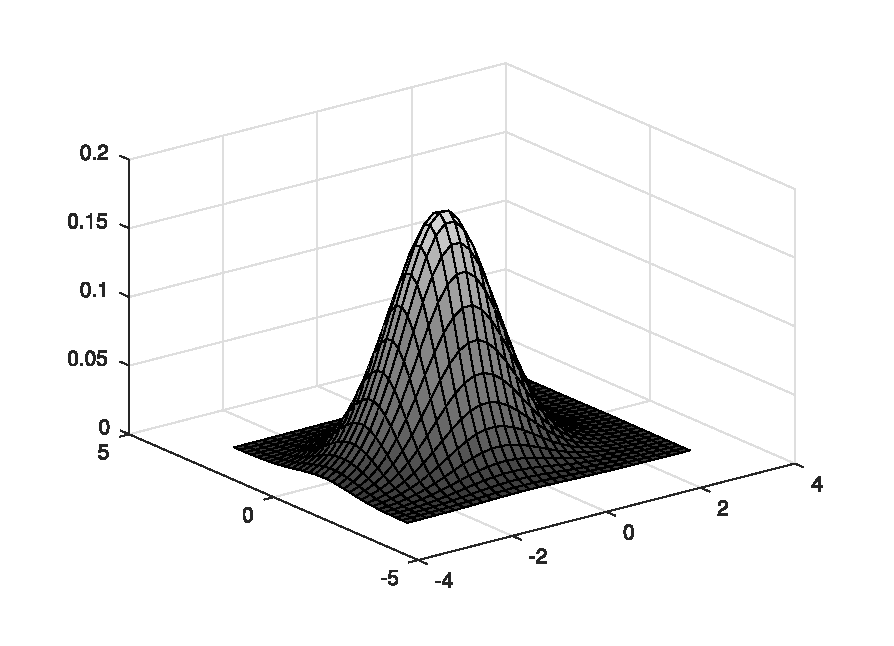
\includegraphics[width=8cm]{bvnpdf_gray.eps}
	\caption{A Bivariate Normal Distribution}
   \label{fig:bvnpdf}
\end{figure}
Given a joint probability distribution of the variables $x_1$ and $x_2$ as:

\begin{equation}
\begin{pmatrix}x_1\\
x_2\\
\end{pmatrix} 
\sim \mathcal{N}\begin{pmatrix} 
\begin{pmatrix}\mu_1\\
\mu_2\\
\end{pmatrix} ,\begin{pmatrix}\sigma_{11} & \sigma_{12}\\
\sigma_{21} & \sigma_{22}\\
\end{pmatrix} 
\end{pmatrix}
\end{equation}

It is possible to get the conditional probability of $x_1 | x_2$ or vice-versa. In a GP, we can derive the posterior from the prior and the observations; it's just that,  we are talking about the joint probability all the values of the function $f(x)$ for all the values of $x$ within the specified bounds.

To sum it up, the posterior is the joint probability of the outcome of the values of the function out of which some are observed (denoted by $f$) and some are not (denoted by $f^*$). 

\begin{equation}
\label{equ:f_f*}
\begin{pmatrix}f\\
{f^*}_2\\
\end{pmatrix} 
\sim \mathcal{N}\begin{pmatrix} 
\begin{pmatrix}\mu\\
\mu_*\\
\end{pmatrix} ,\begin{pmatrix}K & K_*\\
{K_*}^T & K_{**}\\
\end{pmatrix} 
\end{pmatrix}
\end{equation}

Here, $K$ is the matrix we get by applying the kernel function to the observed values, \ie the similarity between each observed $x$ .$K_*$ represents the similarity of the training values to the test values whose output values are to be estimated. $K_{**}$ gives the similarity of the test values with each other. We are ultimately trying to determine $p(f_*|x_*,x,f)$ where $f$ and $f_*$ are jointly distributed as shown in equation \ref{equ:f_f*}. {\color{red}Skipping the proof details}, we ultimately are able to define the distribution $f_* \sim \mathcal{N} (\mu_*,\Sigma_*)$, where $\mu_*$ is the mean and $\Sigma_*$ is the covariance matrix.

\subsection{Gaussian Processes for Machine Learning}
As stated in \cite{rasmussen2003gaussian}, GPs can be used to model system dynamics. Assuming a set of $N$-dimensional observations of the form $(s,a,s')$, we can use separate Gaussian Process model for predicting each coordinate of the system dynamics. For example, the inputs can be the state-action pair $(s,a)$ and the output is a Gaussian distribution over $y = s'_n$, $n = 1,2,...N$. A multivariate Gaussian distribution over the next state and transition probability can be obtained. GPs can be used to model value functions as a function of states. We'd typically specify a finite number of data points $S=s_1,s_2,..s_m$ and let the GP predict it over the space. \par 
In general, a few useful properties of GPs are exploited in order to make them popular in terms of their use in machine learning.

\chapter{The GPQ Algorithm} % Main chapter title

\label{gpq} % Change X to a consecutive number; for referencing this chapter elsewhere, use \ref{ChapterX}
\section{Perception in the loop}
 
 Perception is how the robot is aware of the dynamics of the environment. Just as humans perceive things with their ey es, robots use sensors in order to be aware of its surroundings. Perception usually provides data which allows the robot to determine where it is as well as how far the obstacles or goals or adversaries are. The robot must be able to make intelligent decisions based on the data it gathers. Sensors are very critical for intelligent robots to carry out tasks in dynamic environment which limit and define the capability of a robot \cite{tokekar2014placement}. In order for the robot to be able to navigate through an environment or perform a task of obstacle avoidance it needs to be equipped with sensors which are able to tell what surrounds it.\par 
\textit{Perception in the loop} may be explained with this example. Imagine a robot equipped with a laser sensor (as shown in figure \ref{fig:perception_example}) which provides the distance between the robot and its nearest obstacle essentially informing the robot about its surroundings. The task of the robot is to navigate through this environment without crashing into obstacles assuming the robot has no prior information about the environment and only has access to the real time laser data. How can we use the laser data in order to carry out the task?
\begin{figure}[H]
	\centering
	\includegraphics[width=8cm]{perception_1.pdf}
	\caption {A UAV equipped with a laser sensor}
   \label{fig:perception_example}
\end{figure}

\section{The Simulator setup}caption
\label{sims}
Two simulators were implemented in order to present the idea of perception and subsequently implementing the idea of reinforcement learning in order to learn a \textit{skill}.
\begin{itemize}
\item Simulator 1: A python based obstacle avoidance simulator: As shown in figure \ref{fig:perception_sim_1}, the robot is trying to navigate without colliding with obstacles in a dynamic environment setting. The white obstacles move slower compared to the orange obstacle. The robot is equipped with a laser sensor which uses $6$ beams in order to find out the distances from the obstacles at different angles. The robot has a constant speed and can perform $3$ actions; turn left, turn right or stay in the same direction. 

\begin{figure}[htp]
	\centering
	\includegraphics[width=8cm]{perception_sim_1.png}
	\caption {A python based simulator for obstacle avoidance}
   \label{fig:perception_sim_1}
\end{figure}

\item Simulator 2: A second simulator was implemented in the Gazebo robot simulator~\cite{koenig2004design}. A UAV equipped with a Hokuyo Laser was implemented in the simulator as shown in figure \ref{fig:perception_sim_2}. This may be considered as a $3$D extension of the simulator shown in figure \ref{fig:perception_sim_1}. With infinite state-action space and ability to add robot dynamics, this simulator is a higher fidelity simulator compared to the python-pygame based $2$D simulator. 

\begin{figure}[htp]
	\centering
	\includegraphics[width=8cm]{perception_sim_2.png}
	\caption {A UAV equipped with laser sensor in Gazebo Robot Simulator}
   \label{fig:perception_sim_2}
\end{figure}
\end{itemize}

In both of the above simulators the main principle of \textit{perception in the loop} is used in order to use the laser data to find out the current position of the obstacle with respect to the robot and take an optimal action in order to avoid the obstacle. In order to learn \textit{obstacle avoidance} as a \textit{skill} the algorithm must be agnostic to the shape or size of the obstacle and it should work in case of moving obstacles as well.

\subsection{Laser data and $Q$-Learning}
\label{laser_learning}
In order to learn the \textit{skill} of obstacle avoidance, we decided to learn the mapping from sensor values to action. A naive $Q$-Learning algorithm was implemented (refer to algorithm \ref{q_learning}) on the simulators described in section \ref{sims}. For the python based simulator, any state $s \in S$ is defined as a set of laser sensor values \{$l_1,l_2,l_3,l_4,l_5,l_6$\}, where $l_i \in \mathcal {P} (\mathbb{Z})$ Action $a$ can be chosen from a set of action $A := \{0,1,2\}$ where action = $0$ turns the robot left by a certain angle, action = $1$ turns the robot right by a certain angle and action = $2$ does not change the orientation of the robot. A reward of $-500$ is given on a crash else the reward is an increasing function of the sum of the readings of the $6$ laser sensors. (higher the readings farther the robot is from the obstacle which must be rewarded well.)\par 
In case of the Gazebo Robot Simulator, the state-space $S$ and the action-space $A$ are both continuous spaces. Assuming there are $8$ laser beams, the state $s$ may be represented as \{$l_1,l_2,l_3,l_4,l_5,l_6,l_7,l_8$\}. Here $l_i$ can take any real value from $0$ to $6$. (The Hokuyo sensor is simulated in Gazebo Simulator with a maximum range of $6$ meters.) The action $a$ may be represented as a $3$D vector $x_{\hat{i}} + y_{\hat{j}} + z_{\hat{k}}$. By excluding the robot dynamic constraints from the analysis, we have infinite possible values for a state-action pair $(s,a)$.\par 

Let us consider a static environment first. Assuming each sensor can give $20$ discrete values in case of Simulator $1$ given in section \ref{sims}, we have about $2$ \textit{million} possible states. To observe all of the states in order to be able to store and update the value function (or $Q$ values) is a tedious task. Once a sufficient number of states are observed for the optimal $Q$ values, the robot may learn to navigate through the environment successfully. This may take a longer time due to the size of the state space. In case of simulator $2$, the state space is infinite and hence it is not possible to observe all the possible state-action pairs. 

\section{GPQ Algorithm}
 A Gaussian Process model of the value function ($Q$) is presented in \cite{chowdhary2014off} in both batch and online settings. Consider the problem of finding the value function for over a $million$ state-action pairs in limited time described in section \ref{laser_learning}. The problem here closely relates to the problem in section \ref{GPR} where we were tasked to find out a function to fit the observed data. Given a set of observed state-action pairs $(s,a)$ and the reward $r$, we calculate the $Q$ values for the observed state-action pairs $(s,a)$. Using Gaussian Process Regression (section \ref{GPR}), we predict the $Q$ values over the entire state space $S$ (Refer algorithm \ref{batch_gpq_algorithm}). 
 
 \begin{algorithm}
\label{batch_gpq_algorithm}
\SetKwInOut{Input}{Input}\SetKwInOut{Init}{Initialize}\SetKwInOut{local}{Local data}
\SetKwFunction{trainingPhase}{trainingPhase}\SetKwFunction{findMax}{findMax}\SetKwFunction{batchGPQ}{batchGPQ}\SetKwFunction{updateGP}{updateGP} \SetKwFunction{gpPredict}{gpPredict}

\SetKwProg{training}{}{}{}
\training{\trainingPhase{}}{
\Input{$S$ is a set of states\\$A$ is a set of action}
\local{store the training data $T := \{s,a,r,s'\}$,\\previous state $s$\\previous action $a$\\,current reward $r$\\next state $s'$}
\Init{$T$ $\leftarrow$ empty}
 \For{$i \in (1,N)$}{
        $s \leftarrow$ current state \\
        $a \leftarrow$ random action \\
        Apply $a$ for a $\Delta t$ time\\
        $s' \leftarrow$ observed state\\
        $r \leftarrow $ observed reward\\
        $T \leftarrow T \cup \{(s,a,r,s')\}$
     }
}

\SetKwProg{gpq}{}{}{}
\gpq{\batchGPQ{}}{
\Input{$T:= {(s,a,r,s')}$ is the training set recorded during the training phase}
\Init{Gaussian Process \texttt{GP} with RBF kernel of appropriate length scale}
\While{Termination condition not reached}
{$dX \leftarrow$ \texttt{input to the GP}\\
$tX \leftarrow$ \texttt{output of the GP}.\\
 \For{$i \in (1,N)$}{
 $dX \leftarrow dX \cup {(s_i,a_i)}$\\
 $tX \leftarrow r_i + \findMax(\texttt{GP},s')$
 }
 \updateGP($dX,tX$)
}
}

\SetKwProg{find}{}{}{}
\find{\findMax{\texttt{GP}, $s'$}}{
\Init{$max \leftarrow 0$ }
	\For{$a \in A$}{
		$temp \leftarrow$ \gpPredict($s'$,$a$)\\
        \uIf {temp $>$ max}
        {
        	$max \leftarrow temp$
		}
}
\texttt{return} $max$
}

\caption{Batch GPQ Algorithm}
\end{algorithm}

\chapter{The GP-MFRL Algorithm} % Main chapter title
In this chapter,the use of GP regression to learn the transition function is described and the details about the GP-MFRL algorithm -- the main work of this thesis are provided. The simulator system setup is discussed in the section

\label{gpMfrl} % Change X to a consecutive number; for referencing this chapter elsewhere, use \ref{ChapterX}
\section{Multi-Fidelity Reinforcement Learning}
We build our work upon a recently proposed Multi-Fidelity Reinforcement Learning (MFRL) algorithm by Cutler et al.~\cite{cutler2014reinforcement}. MFRL leverages multiple simulators to minimize the number of real world (\ie, highest fidelity simulator) samples. The simulators denoted by $\Sigma_0,\ldots,\Sigma_D$, have increasing levels of fidelity with respect to the real environment. For example, $\Sigma_0$ can be a simple simulator that models only the robot kinematics, $\Sigma_1$ can model the dynamics as well as kinematics, $\Sigma_2$ can additionally model the wind disturbances, and the highest fidelity simulator can be the real world (Figure~\ref{fig:mfrl_architecture}). 

\begin{figure}[htp]
	\centering
	\includegraphics[width=\textwidth]{mf.eps}
	\caption {MFRL framework: First simulator captures only gridworld movements of a point robot while second simulator has more fidelity using a physics simulator. Control can switch back and forth between simulators and real environment which is essentially the third simulator in the multi-fidelity simulator chain.}
   \label{fig:mfrl_architecture}
\end{figure}

MFRL differs from transfer learning~\cite{taylor2007transfer} where transfer of parameters is allowed only in one direction. The MFRL algorithm starts in $\Sigma_0$. Once it learns an optimal policy in $\Sigma_0$, it switches to a higher fidelity simulator. If it observes that the policy learned in lower fidelity simulator is no longer optimal in the higher fidelity simulator, it either switches back to a lower fidelity simulator or stays at the same level. It was shown that the resulting algorithm has polynomial sample complexity and minimizes the number of samples required from the highest fidelity simulator. 

The original MFRL algorithm uses Knows-What-It-Knows (KWIK) framework~\cite{li2011knows} to learn the transition and reward functions in each level. The algorithm essentially maintains a mapping from a state-action pair to the learned reward and the next state. The reward and the transition for each state-action pair is learned independently of others. While this is reasonable for general agents, in case of planning for robots we can exploit the spatial correlation between neighboring state-action pairs to speed up the learning. Our main contribution in this paper is to show how to use Gaussian Process (GP) regression to learn the transition function in an MFRL framework using fewer samples. 

GPs are commonly used to learn transition models for agents moving in the real world~\cite{Dames2015} and have been used in RL to learn the transition function~\cite{rasmussen2003gaussian}, the reward function~\cite{deisenroth2010efficient} and the value function~\cite{engel2005reinforcement}. GPs can predict the learned function for any query state-action pair, and not just for the discretized set of state-action pairs used when planning. In MFRL, the state space of $\Sigma_i$ is a subset of the state space of $\Sigma_j$ for all $j>i$. Therefore, when the MFRL algorithm switches from $\Sigma_i$ to $\Sigma_{i+1}$ it already has an estimate for the transition function for states in $\Sigma_{i+1}\setminus\Sigma_{i}$. Thus, GPs are particularly suited for MFRL which we verify through our simulation results.


\section{Learning Transition Dynamics as a GP}
A Markov Decision Processes (MDP)~\cite{puterman2014markov} is defined by a tuple: $\langle S,A,\mathcal{R}_{ss'}^a,\mathcal{P}_{ss'}^a,\gamma\rangle$. $S$ and $A$ are the set of states and actions respectively. $\mathcal{R}_{ss'}^a$, referred to as reward dynamics, defines the reward received by the agent in making a transition from state $s$ to $s'$ while taking action $a$ and $\mathcal{P}_{ss'}^a$ is the probability of making this transition (also referred to as transition dynamics). 

Generally the agent does not know the reward it will receive after making a transition nor does it know the next state it will land in. The agent learns these parameters through interactions with the environment which is subsequently used to plan an optimal policy to earn the maximum expected reward, \ie, $\pi^{*}:S \rightarrow A$.

RL algorithms are broadly classified into \emph{model-free} learning and \emph{model-based} learning as seen in section \ref{rl}. Approaches that explicitly learn transition dynamics and/or reward dynamics of an environment are known as model-based learning \cite{brafman2002r,kearns2002near}. The learned transition and reward dynamics can then be used to find the optimal policy using, for example, policy iteration or value iteration~\cite{sutton1998reinforcement} which are often referred to as \emph{planners}. In contrast, Strehl et al.~\cite{strehl2006pac} presented a model-free algorithm wherein the agent directly learns the value function and obtains the optimal policy. In this paper, we focus on model-based approaches and use GP regression to learn the transition dynamics. 

Rasmussen and Kuss~\cite{rasmussen2003gaussian} showed how to use GPs for carrying out model-based RL. They assumed that the reward dynamics are known and the transition and value function was modeled as a GP. We use the same assumption for ease of exposition. However, assuming reward dynamics to be known is not a critical requirement. In fact, reward dynamics can also be easily be modeled as GPs.

\begin{figure}[htp]
	\centering
	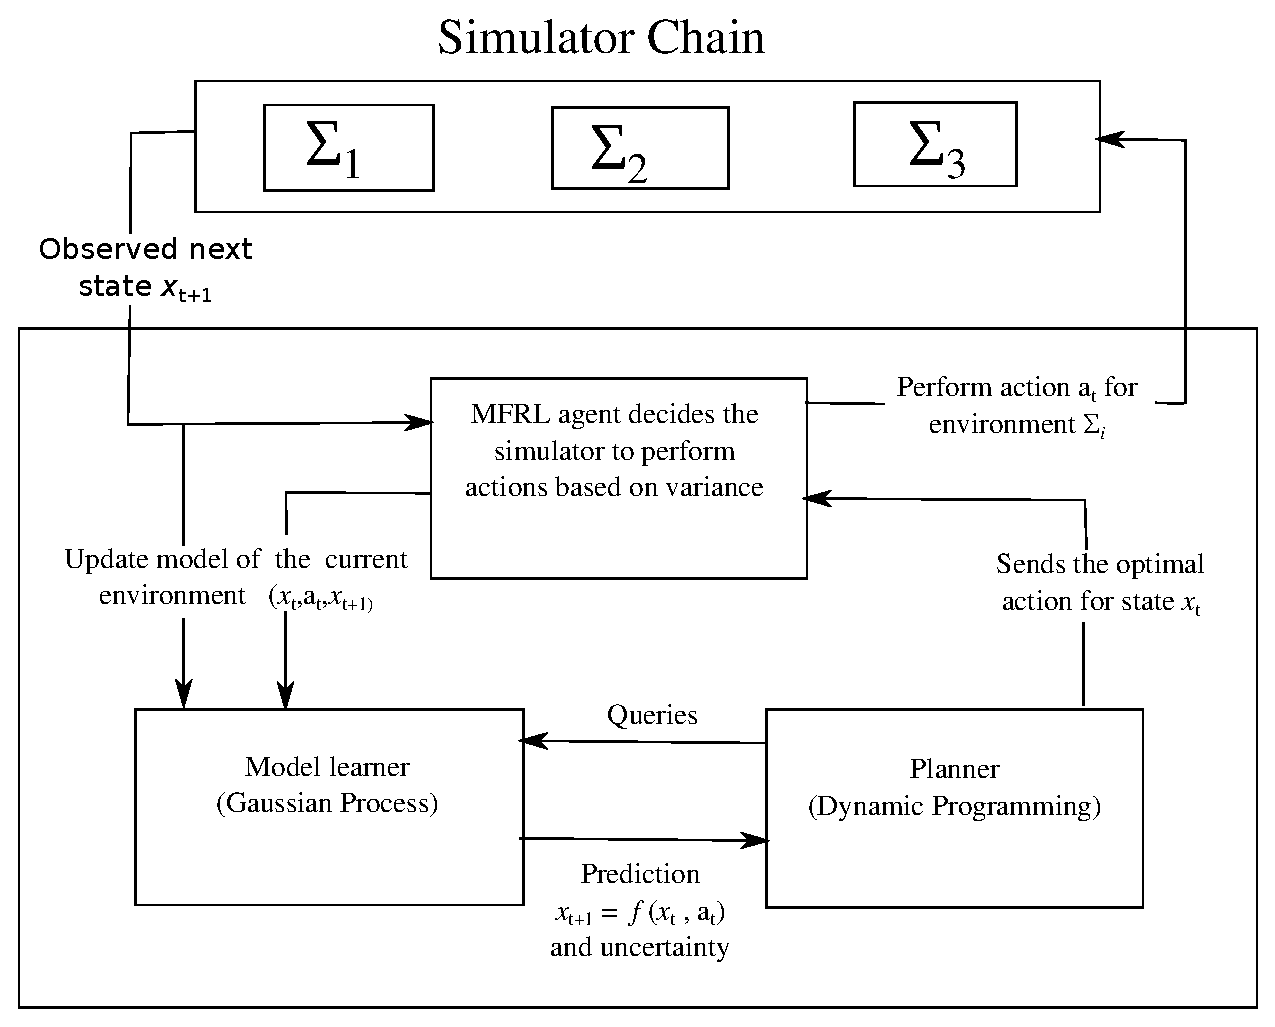
\includegraphics[width=8cm]{gp-mfrl.eps}
	\caption {Overview of the GP-MFRL algorithm }
   \label{fig:gp_mfrl_system}
\end{figure}

We observe a number of transitions: $\mathcal{D} = \{(\textbf{x}_t, a_t, \textbf{x}_{t+1})\}$. Let $\textbf{x}_{t+1} = f(\textbf{x}_t, a_t)$ be the (unknown) transition function that must be learned. Our goal is to learn an estimate $\tilde{f}(\textbf{x}, a)$ of $f(\textbf{x}, a)$ in as few samples in $\mathcal{D}$ as possible. We can then use this estimated $\tilde{f}$ for unvisited state-action pairs (in place of $f$) during value iteration to learn the optimal policy. $f$ can also be a stochastic transition function, in which case, the GP estimate gives the mean and the variance of this noisy transition function. For a given state-action pair $(s,a)$, the estimated transition function is defined by a normal distribution with mean and variance given by:
\begin{equation}\label{gaussian_mean}
\mu_{(s,a)|\mathcal{D}} = \mathcal{K}_{(s,a)\mathcal{D}}\mathcal{K}^{-1}_{\mathcal{D}\mathcal{D}}\vec{\mathcal{X}}_{\mathcal{D}} 
\end{equation}
\begin{equation}\label{gaussian_variance}
\sigma^2_{(s,a)|\mathcal{D}} = \mathcal{K}\{(s,a),(s,a)\}-\mathcal{K}_{(s,a)\mathcal{D}}\mathcal{K}^{-1}_{\mathcal{D}\mathcal{D}}\mathcal{K}_{(s,a)\mathcal{D}}
\end{equation}
where $\mathcal{K}$ is the kernel function.

GP regression requires a kernel which encodes the correlation between the values of $f$ at two points in the state-action space. Choosing a right kernel is the most crucial step in implementing GP regression. We choose the Radial Basis Function (RBF) kernel for our implementation since it models the spatial correlation we expect to see in an aerial robot system well. However, any appropriate kernel can be used in our algorithm depending on the environment to be modeled. 

RBF has infinite dimensional feature space and satisfies the Lipschitz smoothness assumption. It can be defined as follows: for two points $\textbf{x}$ and $\textbf{x'}$,
\begin{equation} \label{kernel_def}
\begin{split}
k(\textbf{x}, \textbf{x'})= \exp\bigg(-\frac{|| \textbf{x}-\textbf{x'}||^2}{2\sigma^2}\bigg)\end{split}
\end{equation}
where $||\textbf{x}-\textbf{x'}||^{2}$ is the squared Euclidean distance and $\sigma$ is a hyperparameter for the kernel often known as \textit{characteristic length-scale}. Here, $\textbf{x}$ represents a point in the joint state-action space.

Instead of using GPs to predict the next state, we use it to predict the velocity with which the robot will move when a given action $a_t$ is applied at a state $s_t$. Learning the velocity vector helps in transitioning between simulators as the size of the state space itself may be different. For example, one can construct a multi-fidelity simulator where $\Sigma_0$ is a $n\times n$ grid, $\Sigma_1$ is a denser $2n\times 2n$ grid, and so on. An action in $\Sigma_0$ moves the robot one unit whereas the same action in $\Sigma_1$ moves the robot only 0.5 units. By learning the velocity instead of the next state, we can scale the learned velocity function to easily compute the transition function in any $\Sigma_i$ as:
\begin{equation} \label{velocity_def}
\begin{split}
\vec{\mathcal{V}} \ (s_t,a_t) = \frac{s_{t+1}-s_t}{\Delta_i} 
\end{split}
\end{equation}
where $\Delta_i$ is the time scaling of a simulator. If the state spaces of all simulators are the same, then one can use GPs to predict the next state instead of the velocity vector.

We train two GP regressions, $f_x,f_y:\mathbb{R}^4\rightarrow\mathbb{R}$, assuming independence between the two output dimensions. Let $(x_i,y_i)$ be the current state of the agent. Actions actions are represented using a tuple $(a_x,a_y)$ where $a_x$ and $a_y$ can take the values between $0$ or $1$. 

The GP prediction is used to determine the transitions, $(x_i,y_i,a_x)$ $\rightarrow$ $x_{i+1}$ and $(x_i,y_i,a_y)$ $\rightarrow$ $y_{i+1}$ where $(x_{i+1},y_{i+1})$ is the predicted next state with variance $\sigma_x$ and $\sigma_y$ respectively. Value of hyperparameters is estimated by gradient descent by optimizing the maximum likelihood estimate of a training data set. 


\section{GP-MFRL Algorithm}

Using multiple approximations of real world environments has previously been considered in the literature~\cite{abbeel2006using,taylor2007transfer}. Cutler et al. used model-based R-Max algorithm to reduce the number of samples using MFRL framework \cite{cutler2014reinforcement}. We use GP regression to further bring down the empirical sample complexity of MFRL framework. 


Algorithm~\ref{GP-MFRL} gives the details of the proposed framework. As illustrated in Figure~\ref{fig:gp_mfrl_system}, there are two main components of GP-MFRL: (1) Model Learner; and (2) Planner. The model learner in our case is the GP-regression described in the previous subsection. We use value iteration~\cite{sutton1998reinforcement} as our planner to calculate the optimal policy on learned dynamics of environment. 

An \emph{epoch} measures the time span between two consecutive switches in the simulators. Before executing an action, the agent checks (Step 4) if it has a sufficiently accurate estimate of the transition dynamics for the current state-action pair in the lower fidelity simulator, $\Sigma_{d-1}$. If not, it switches to $\Sigma_{d-1}$ and executes the action in the potentially less expensive environment. The function $\rho^{-1}$ checks if the current state is also a valid state in the lower fidelity simulator. 

We also keep track of the variance of the $\mathcal{L}$ most recently visited state-action pairs in the current epoch. If the running sum of the variances is below a threshold (Step 8), this suggest that the robot has found a good policy in the current simulator and it must advance to the next higher fidelity simulator.

Steps 12--16 in describe the main body where the agent computes the optimal action, executes it, and records the observed transition in $\mathcal{D}$. The GP model is updated after every $n_U$ iterations (Step 17). In the update, we recompute the hyper-parameters until they converge.

A new policy is computed every time the robot reaches the goal state (Step 21). If the robot is in the highest fidelity simulator, we also check if the policy has converged by checking if the maximum change in the value function is less than a threshold (Step 22). If so, we terminate the learner.
\pagebreak

\addtolength{\topmargin}{-.875in}

\begin{algorithm}

\SetKwData{Left}{left}\SetKwData{This}{this}\SetKwData{Up}{up}
\SetKwFunction{Learner}{Learner}\SetKwFunction{Planner}{Planner}\SetKwFunction{UpdateGP}{UpdateGP}\SetKwFunction{epochLength}{epochLength}
\SetKwInOut{Input}{Input}\SetKwInOut{Output}{Initialize}
\Input{A simulator chain,\\ Confidence parameter $\psi$ for $(s,a)$,\\ History Length $\mathcal{L}$, \\ Confidence $\Psi$, \\ State mapping $\rho$, \\ Reward dynamics $\mathcal{R}_{ss'}^a$ \\ Update rate $n_U$ }
\Output{Transition dynamics $\mathcal{P}_{ss'}^a$ ; \\ $d = 1$ ;\\ $\mathcal{V}^{*}_d(s) \leftarrow $  \Planner ($\mathcal{P}_{ss'}^a$)}
%\BlankLine
%\KwData {text}
%\emph{special treatment of the first line}\;
\SetKwProg{myalg}{}{}{}
\myalg{\Learner{}}{
\While{\textnormal{true} }{
\emph{$a^{*}_t \leftarrow \underset{}{\textnormal{argmax}_a}$ $\mathcal{V}^{*}_d(s_t)$} \;
\If(\tcp*[h]{Return to level $d - 1$}){$\sigma(\rho^{-1}(s_t,a^{*}_t) \geq \psi \ \bigwedge \ d > 1 $}{\label{lt}
%\lIf{\Left $<$ \This}{\Union{\Left,\This}}
%\lElse{\Union{\This,\Left}}
\emph{$d \leftarrow d-1$}\;
\epochLength $\leftarrow \ 0$
}
%\tcp*[h]{Path length covered $\leftarrow$ 0}
\If{$\sum_{i = t - \mathcal{L}}^{t-1}\sigma(s_i, a_i^{*}) \leq \Psi \  \bigwedge  \epochLength \geq \mathcal{L}$}{\label{forins}
$d \leftarrow d + 	1$ \ (Move up the simulator) \;
\epochLength $\leftarrow \ 0$ \; }

$a^{*}_t \leftarrow {\textnormal{argmax}_a}$ $\mathcal{V}^{*}_d(s_t)$\;
\emph{\textnormal{Execute}  $a^{*}_t $ \textnormal{and store observed} $s_{t+1}, r_{t+1}$ \;
\epochLength $++$ \;
$\mathcal{D}_t=\mathcal{D}_t \cup (s_{t}, \ a^{*}_t  , \ s_{t+1})$}\; 
$s_{t} \leftarrow s_{t+1}$ \;
\If{\epochLength \textnormal{is multiple of $n_U$}  }{\label{forins1}
\emph{$\mathcal{P}^a_{ss'} \leftarrow \UpdateGP(\mathcal{D}_t) $}\;}

\If{ $s_t$ \textnormal{is Goal state}}{\label{forins2}
\emph{$\mathcal{V}_f(s) \leftarrow \Planner(\mathcal{P}_{ss'}^a)$} \;

\If{ \textnormal{${\textnormal{max}_s} \ \mathcal{V}_f (s) - \mathcal{V}_0 (s) \leq 10 \ \% \bigwedge d == D$}}{\label{forins3}
break the loop \;
}
$\mathcal{V}_0 (s) \leftarrow \mathcal{V}_f $\;
}

$t \leftarrow t + 	1$ \;


%}

%\lForEach{element $e$ of the line $i$}{\FindCompress{p}}
}}
\SetKwProg{myproc}{}{}{}
\myproc{\Planner{}}{
%\Input{Reward dynamics $\mathcal{R}_{ss'}^a$ }
\Output{$\mathcal{V}(s)=0, \ \forall (s,a)$ \\ $\Delta = \infty$}
\While{$\Delta > 0.1$}{\label{forins4}
\For{every s:}{
\emph{$temp \leftarrow \mathcal{V}(s) $} \;
\emph{$\mathcal{V}(s) \leftarrow   \textnormal{max}_a \sum_{a} \sum_{s'} \mathcal{P}_{ss'}^a[\mathcal{R}_{ss'}^a+\gamma  \mathcal{V}(s')] $}\;
\emph{$\Delta \leftarrow \textnormal{max}(0, \  |temp - \mathcal{V}(s)Init|)$}
}
}
\emph{return $\mathcal{Q}(s,a)$}
}
\caption{GP-MFRL Algorithm}\label{GP-MFRL}
\end{algorithm}



\section{Simulation Results} \label{gp-mfrl-sim}
We demonstrate the GP-MFRL algorithm in a simulator chain consisting of a virtual gridworld environment and the Gazebo robot simulator~\cite{koenig2004design}. The setup is shown in Figure \ref{fig:gp_mfrl_setup}. The simple grid-world agent operates in a $21\times 21$ grid. The agent receives a reward of $+50$ at the goal location, and $-1$ for all other states. If the agent hits the obstacles, it gets the reward of $-20$. In each time step, an agent can move in one of the four directions viz. up, down, left and right. We add a Gaussian noise of $\sigma$ to the actual transition to represent stochastic environments. The Gazebo simulation setup consists of a quadrotor with PX4 autopilot running in software--in--the--loop (SITL) mode. The PX4 SITL interfaces with the Robot Operating System~\cite{quigley2009ros} via the \texttt{mavros} node. 

The code is written in python and uses scikit-learn \cite{scikit-learn} to implement GP-regression. The code is available online at \url{https://github.com/raaslab/gp_gazebo}.

\begin{figure}[htp]
	\centering
	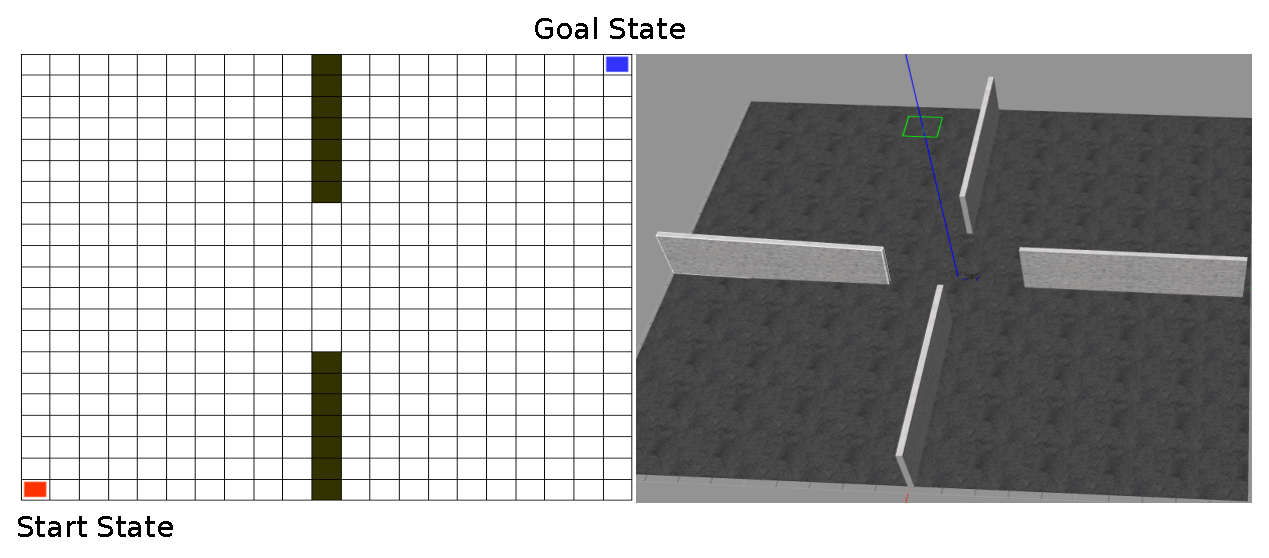
\includegraphics[width=1\columnwidth]{env.eps}
	\caption{The environment setup for a multi-fidelity simulator chain. The simple gridworld environment has two wall obstacles whereas the gazebo environment has four wall obstacles as shown.}
   \label{fig:gp_mfrl_setup}
\end{figure}

Figure~\ref{fig:epoch_samples} shows the switching between the simulators for one run of the GP-MFRL algorithm on the environment shown in Figure~\ref{fig:gp_mfrl_setup}. It can be seen that the agent switches back and forth between the two simulators unlike unidirectional transfer learning algorithms. In the rest of the simulations we study the effect of the parameters used in GP-MFRL and the fidelity of the simulators on the number of samples till convergence.
\begin{figure}[htp]
	\centering 
    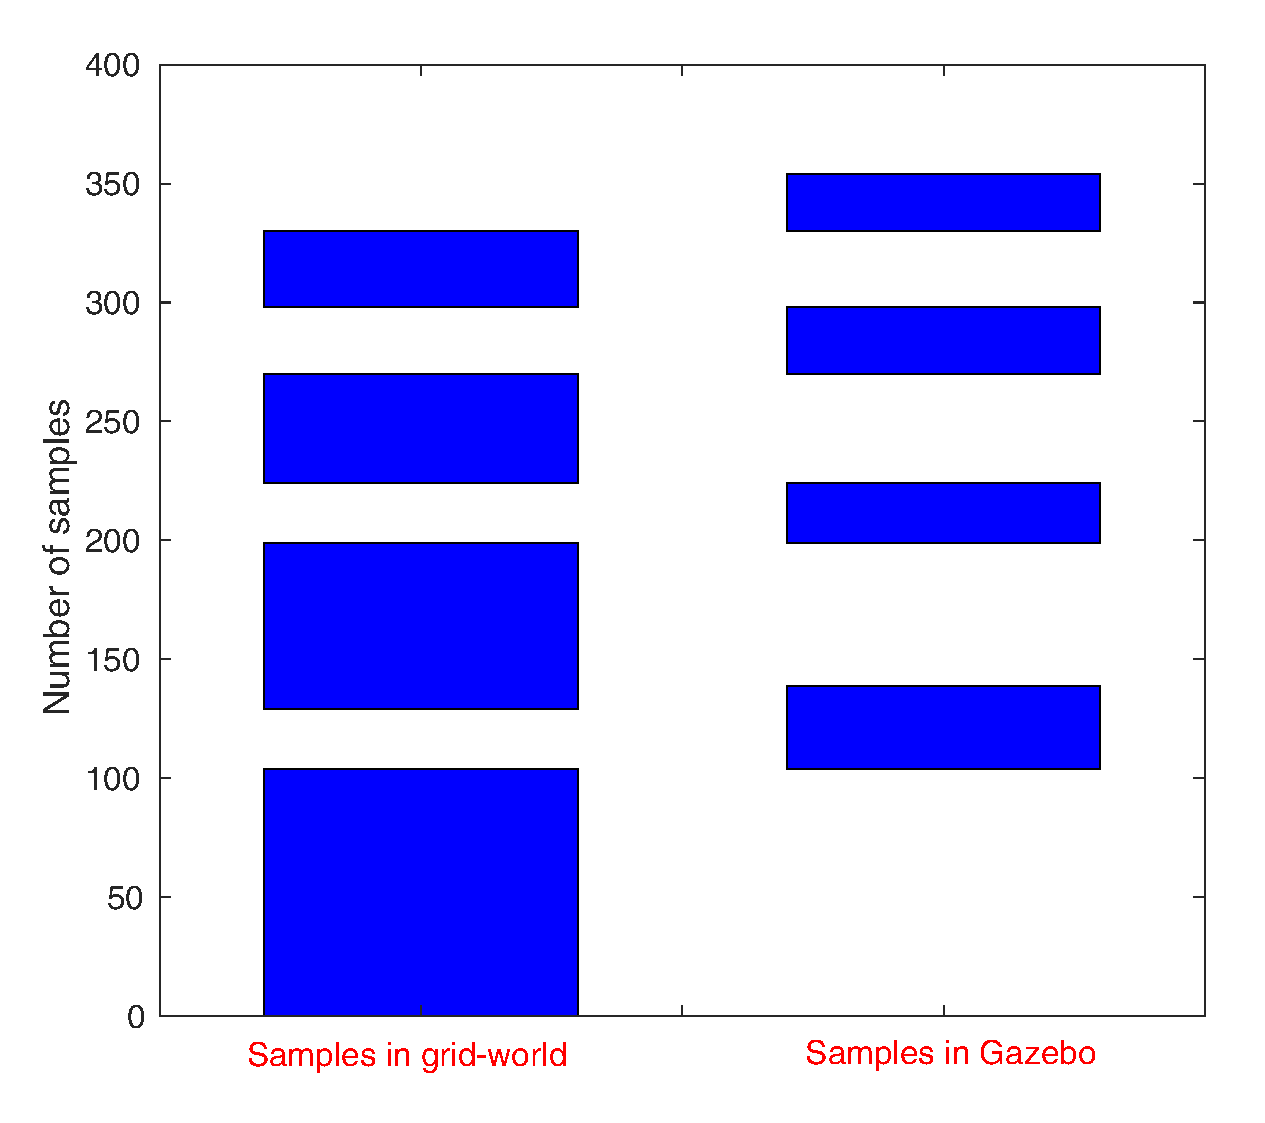
\includegraphics[width=6cm]{epoch.eps}
	\caption{ The figure represents the samples collected in each level of simulator for a $21 \times 21$ grid in a simple grid-world and Gazebo environments. $\Psi$ and $\psi$ were kept 0.4 and $0.1$}
   \label{fig:epoch_samples}
\end{figure}

\subsection{Representative simulations}
We first present three representative scenarios to observe the qualitative performance of the GP-MFRL algorithm. Specifically, we consider three instances and show how the variance evolves over time as more samples are collected. Recall that the main advantage with using GPs is that it allows for quick generalization of observed samples to unobserved state-action pairs.

To demonstrate how variance of the predicted transition dynamics varies from the beginning of experiment to convergence, we plot ``heatmaps'' of the variance. The GP prediction for a state-action pair also gives the variance, $\sigma_x$ and $\sigma_y$, respectively for the predicted state. The heatmap shows $\sqrt{\sigma_x^2 + \sigma_y^2}$ for the optimal action at every state as returned by the Planner. 

Figures~\ref{fig:heatmap1} and \ref{fig:heatmap2} show the heatmaps at the start and convergence for the same environment but with different start and goal positions. As expected, the variance along the optimal (\ie, likely) path is low whereas the variance for states unlike to be on the optimal path from start to goal remains high. 

\begin{figure}
	\centering
    \subfigure[After Initial Training]{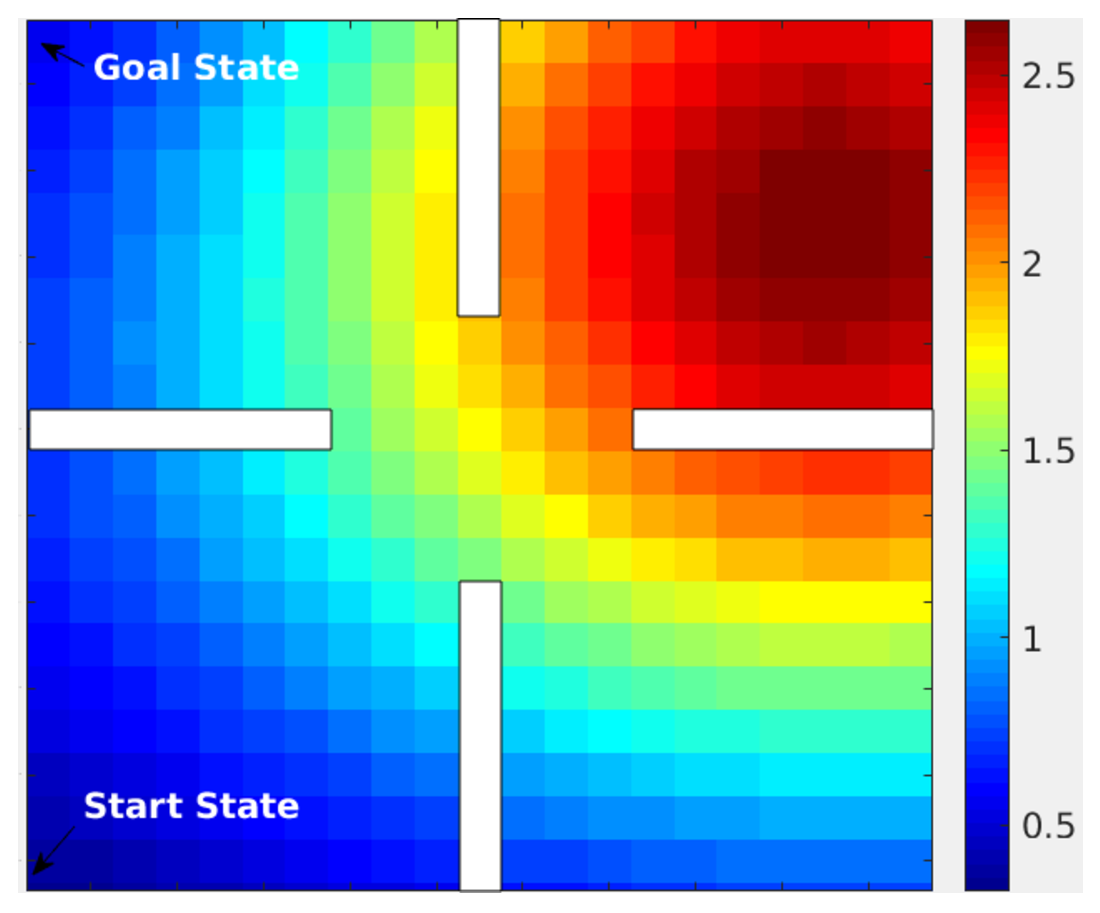
\includegraphics[width=4cm]{heat_init_same.eps}}
    \subfigure[After Convergence]{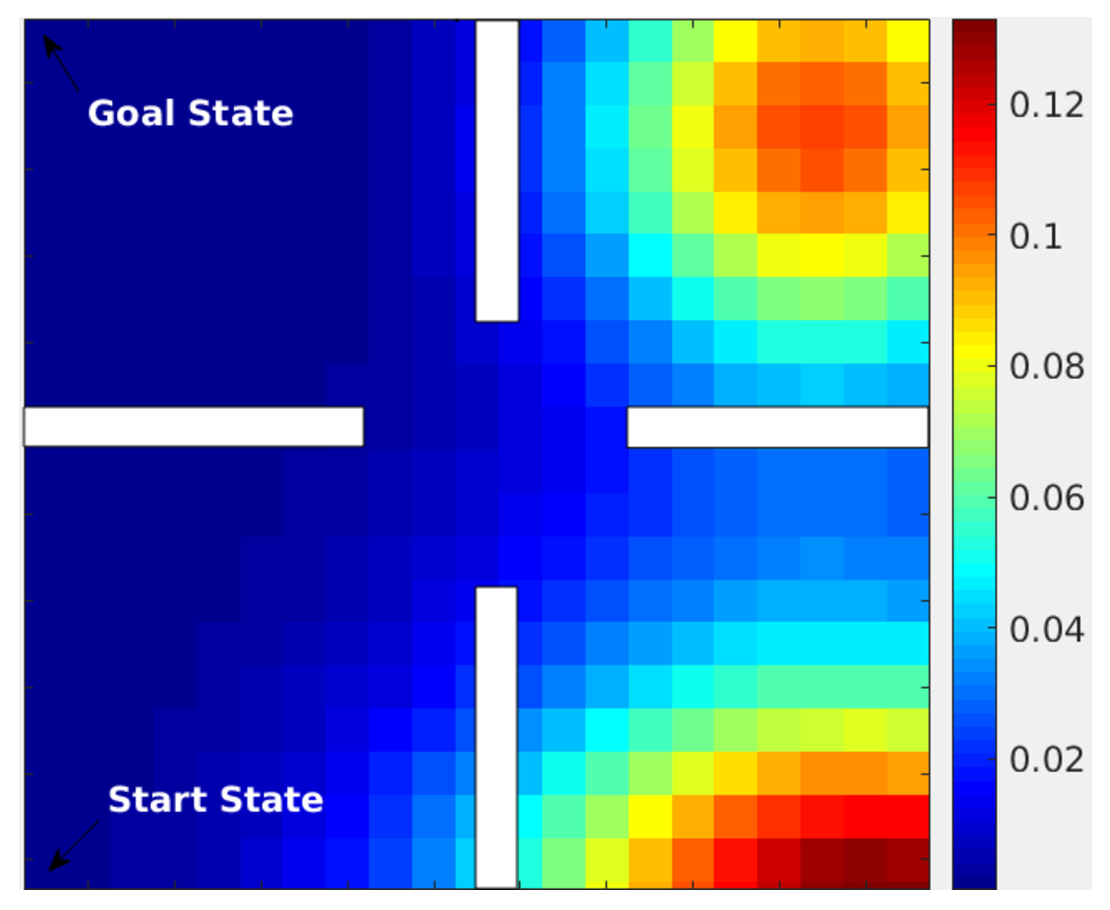
\includegraphics[width=4cm]{heat_same.eps}}
	\caption{Variance plot for $21 \times 21$ multi-fidelity environment after transition dynamics initialization and after algorithm has converged}
   \label{fig:heatmap1}
\end{figure}

\begin{figure}[htp]
	\centering 
    \subfigure[After Initial Training]{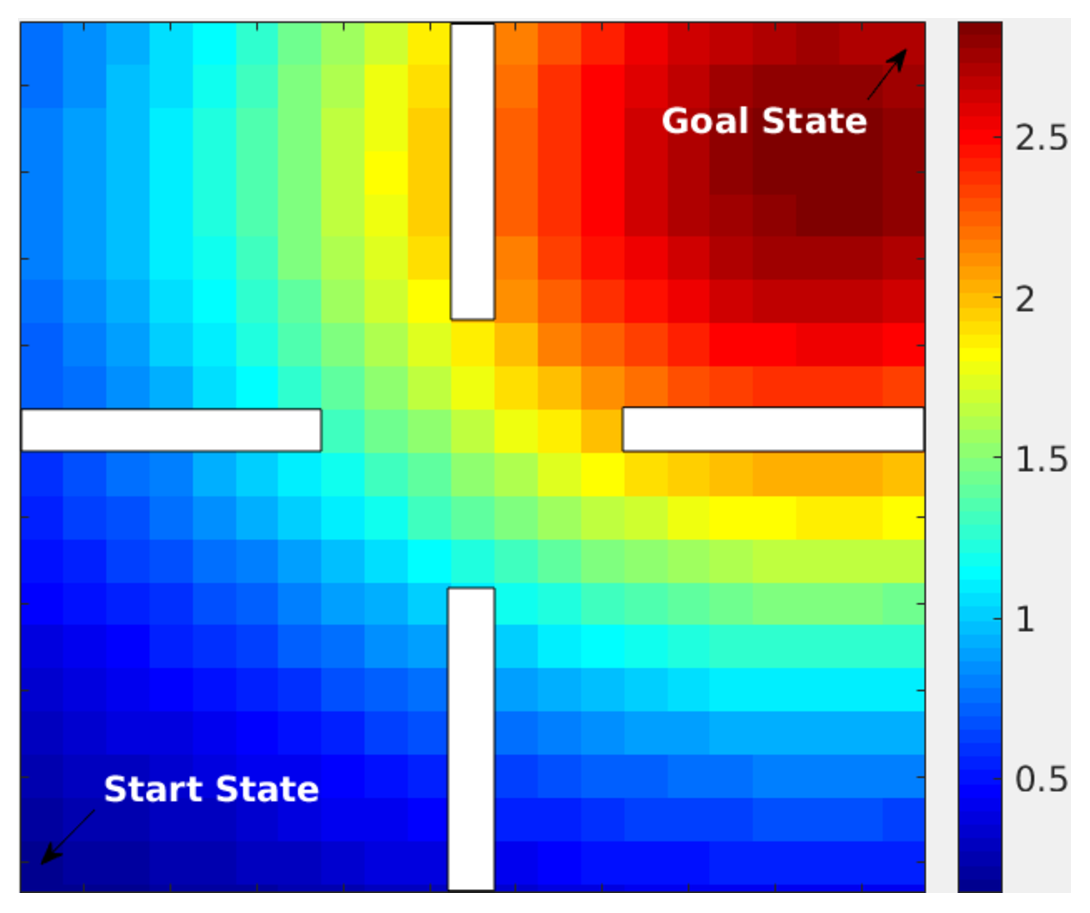
\includegraphics[width=4cm]{heat_init_opposite.eps}}
    \subfigure[After Convergence]{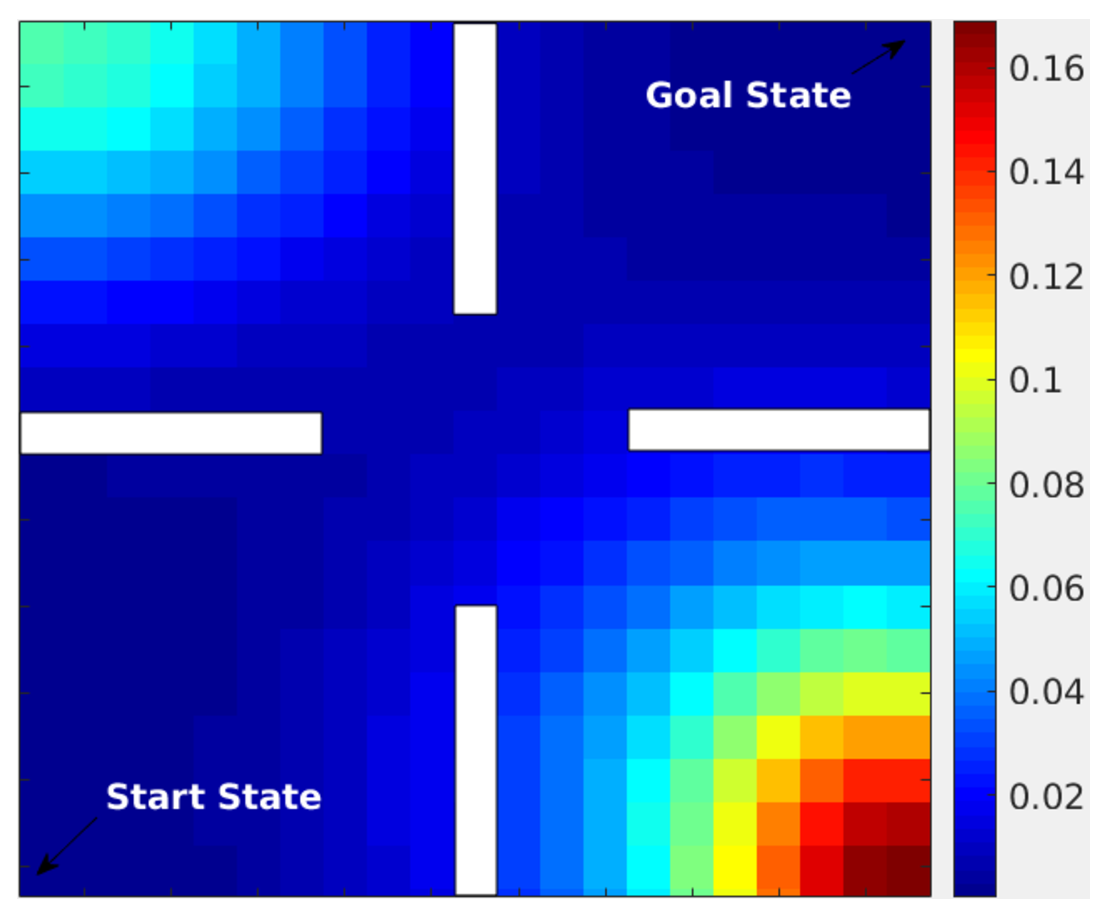
\includegraphics[width=4cm]{heat_opposite.eps}}
	\caption{Variance plot for $21 \times 21$ multi-fidelity environment after transition dynamics initialization and after algorithm has converged}
   \label{fig:heatmap2}
\end{figure}

A more interesting case is presented in Figure \ref{fig:heatmap_four_walls_complex}. Even though there's a path available to reach the goal from the right of wall A, the agent explores that region less than the region near the walls B, C and D (indicated in dark blue showing less variance). This is due to the fact that, the transition dynamics learned in the lower fidelity simulator is used in the higher fidelity simulator leading to lesser exploration of the regions which are not along the optimal path.
\begin{figure}[htp]
	\centering 
	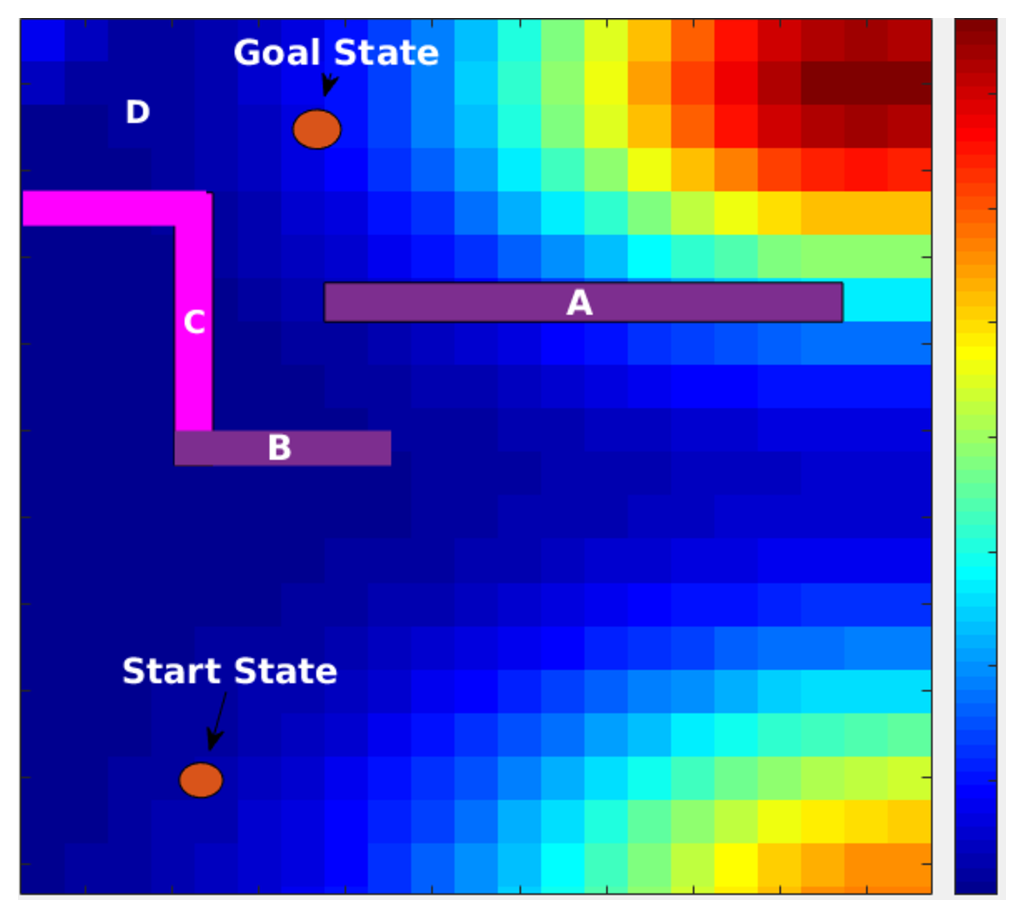
\includegraphics[width=6cm]{heatmap_new.eps}
	\caption{Variance plot for $21 \times 21$ multi-fidelity environment after the algorithm has converged. Walls A and B are only present in the grid-world simulator, whereas all four walls are present in the Gazebo simulator.}
   \label{fig:heatmap_four_walls_complex}
\end{figure}


\subsection{Effect of fidelity on the number of samples.}

We first study the effect of varying fidelity on the total number of samples and the fraction of the samples collected in the higher fidelity simulator. Our hypothesis is that having learned the transition dynamics in the gridworld, the agent will need fewer samples in the higher fidelity Gazebo simulator to find the optimal policy. However, as the fidelity of the first simulator decreases, we would need more samples in Gazebo. 

In order to validate this hypothesis, we varied the noise parameter used to simulate the transitions in the gridworld. The transition model in Gazebo remains the same. The total number of samples collected increases as we increase the noise in gridworld (Figure \ref{fig:gp_mfrl_samples}). As we increase the noise in the first simulator, the agent learns less accurate transition dynamics leading to collection of more number of samples in the higher fidelity simulator. Not only does the agent need more samples, the ratio of the samples collected in the higher fidelity simulator to the total number of samples also increases (Figure \ref{fig:gp_mfrl_ratio}). 


\begin{figure}[htp]
	\centering
	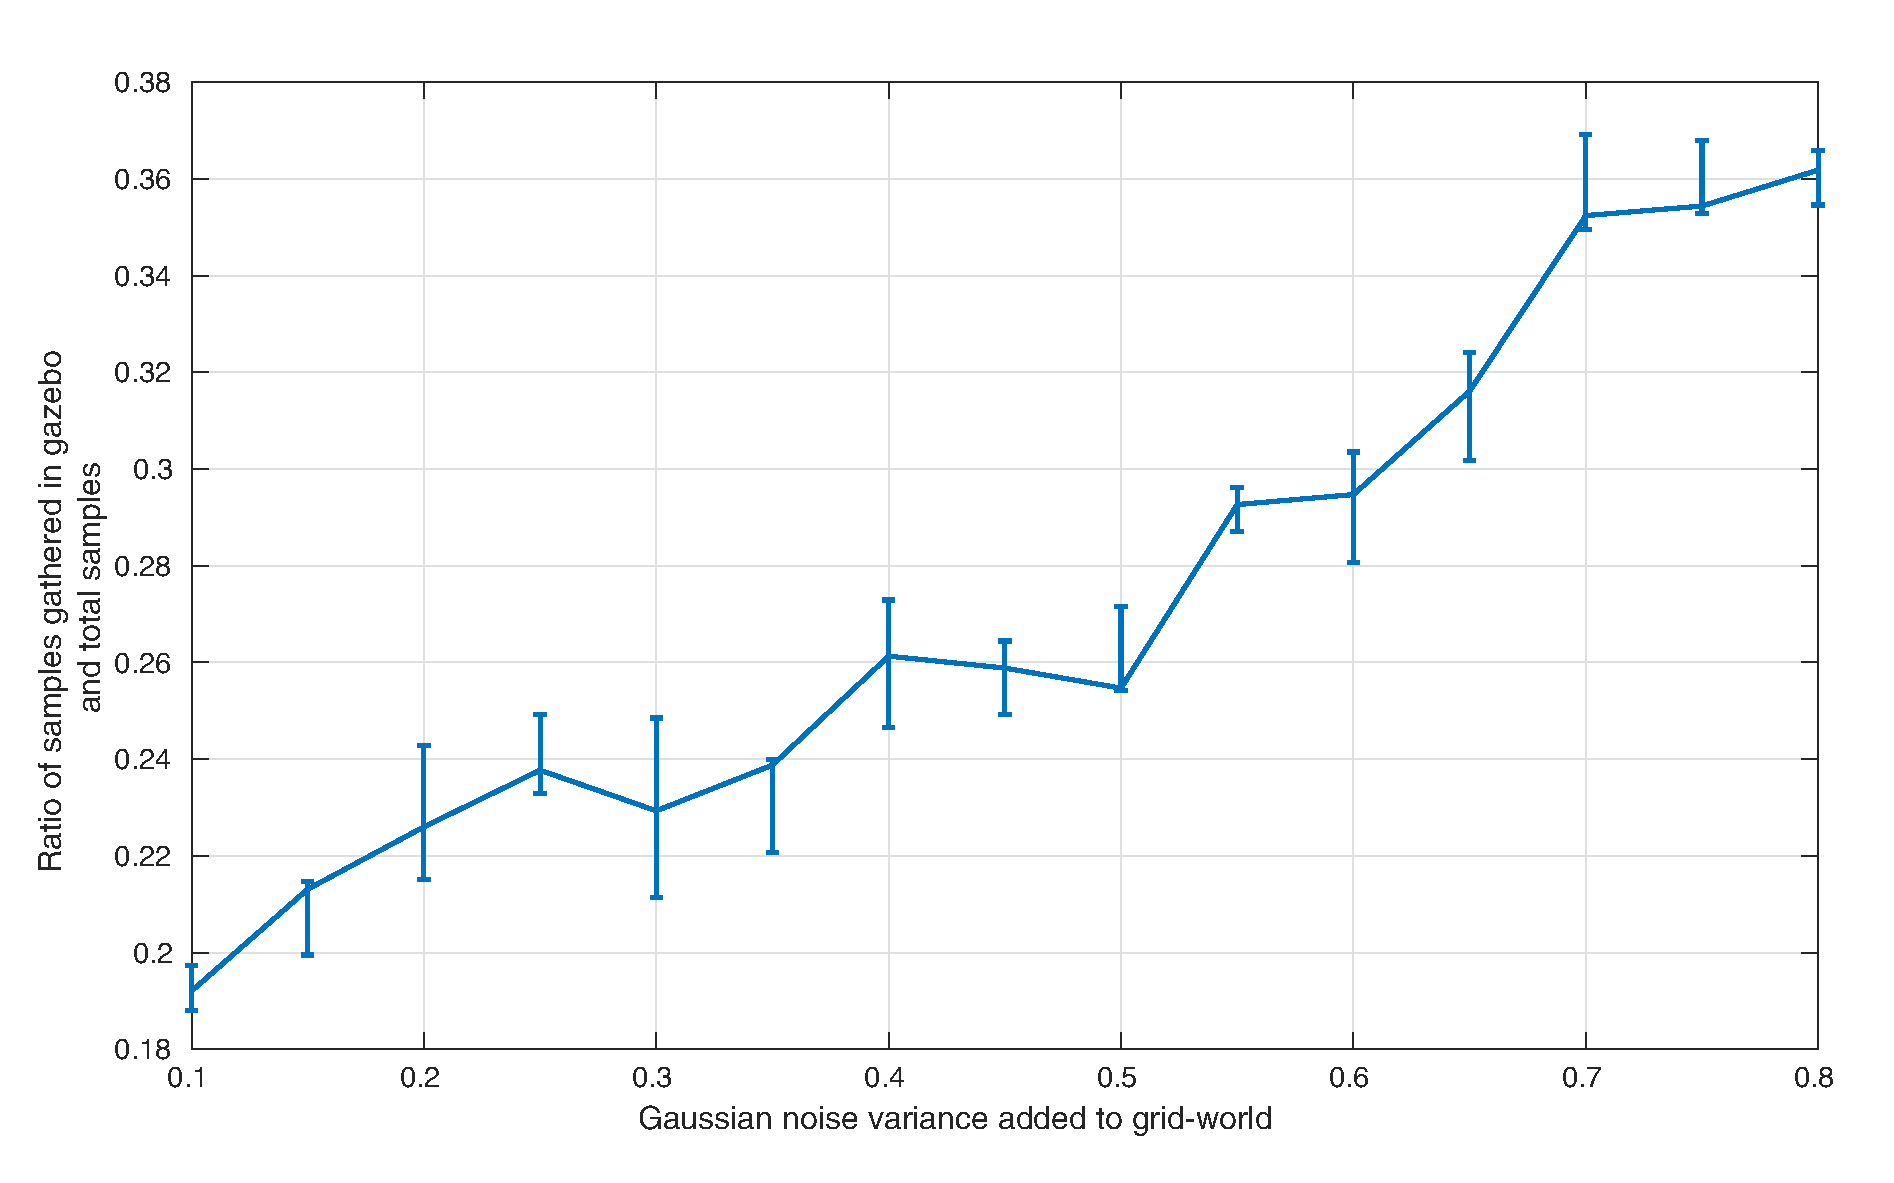
\includegraphics[width=8cm]{ratio.eps}
	\caption{As we make first simulator more inaccurate by adding noise, the agent tends to gather more samples in second simulator }
   \label{fig:gp_mfrl_samples}
\end{figure}

\begin{figure}[htp]
	\centering
	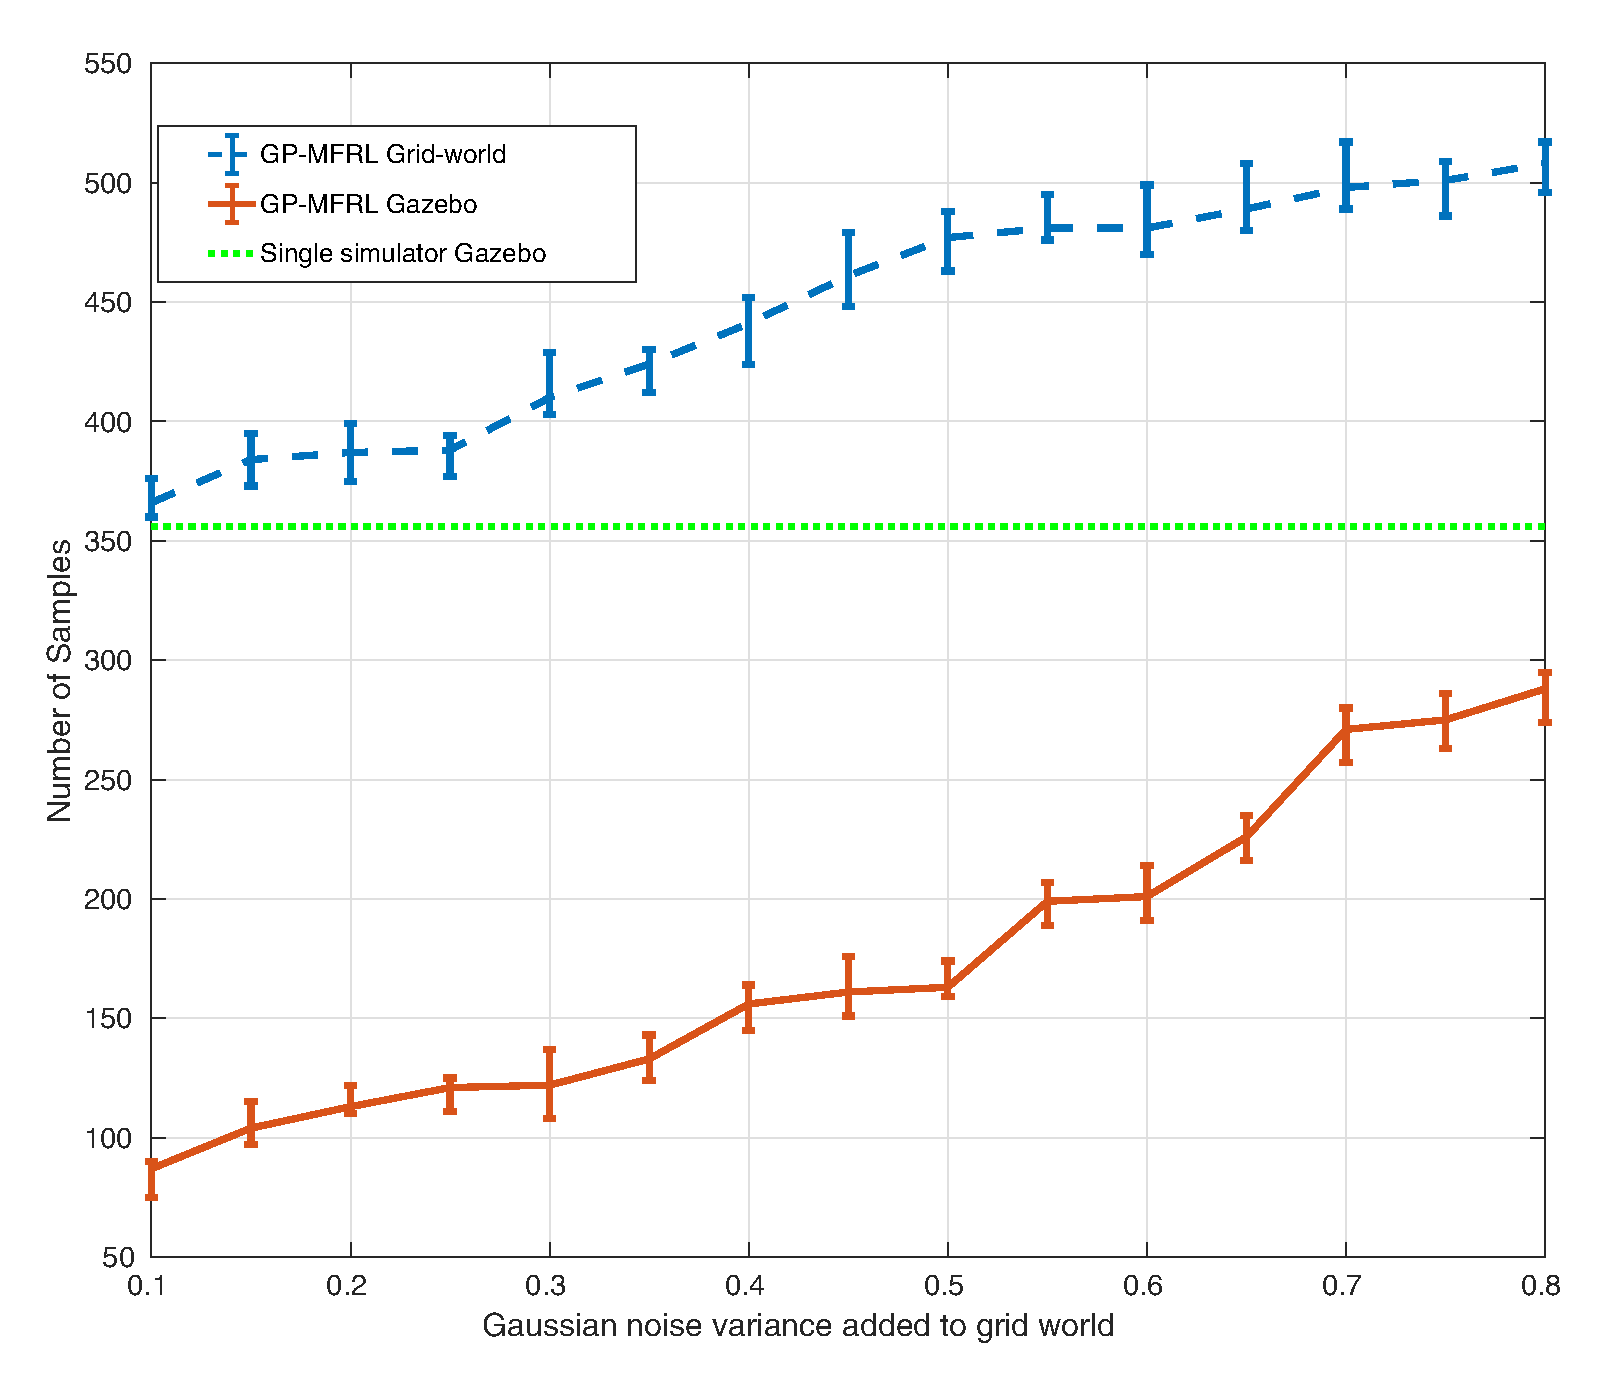
\includegraphics[width=8cm]{samples_gathered_.eps}
	\caption{Ratio of samples gathered in the second simulator to the total samples gathered increases with inaccuracy in the first simulator. The reference line depicts the average number of samples gathered over $10$ runs when only Gazebo simulator was present.}
   \label{fig:gp_mfrl_ratio}
\end{figure}

\subsection{Effect of the confidence parameters.}
The GP-MFRL algorithm uses two confidence parameters, $\psi$ and $\Psi$, which are compared against the variance in the transition dynamics to switch to a lower and higher simulator, respectively. Figure~\ref{fig:threshold} shows the effect of varying the two parameters on the ratio of number of samples gathered in the Gazebo simulator to the total number of samples. As expected, increasing $\psi$ or decreasing $\Psi$ leads to more samples being collected in the higher fidelity simulator. 

\begin{figure}[htp]
	\centering
	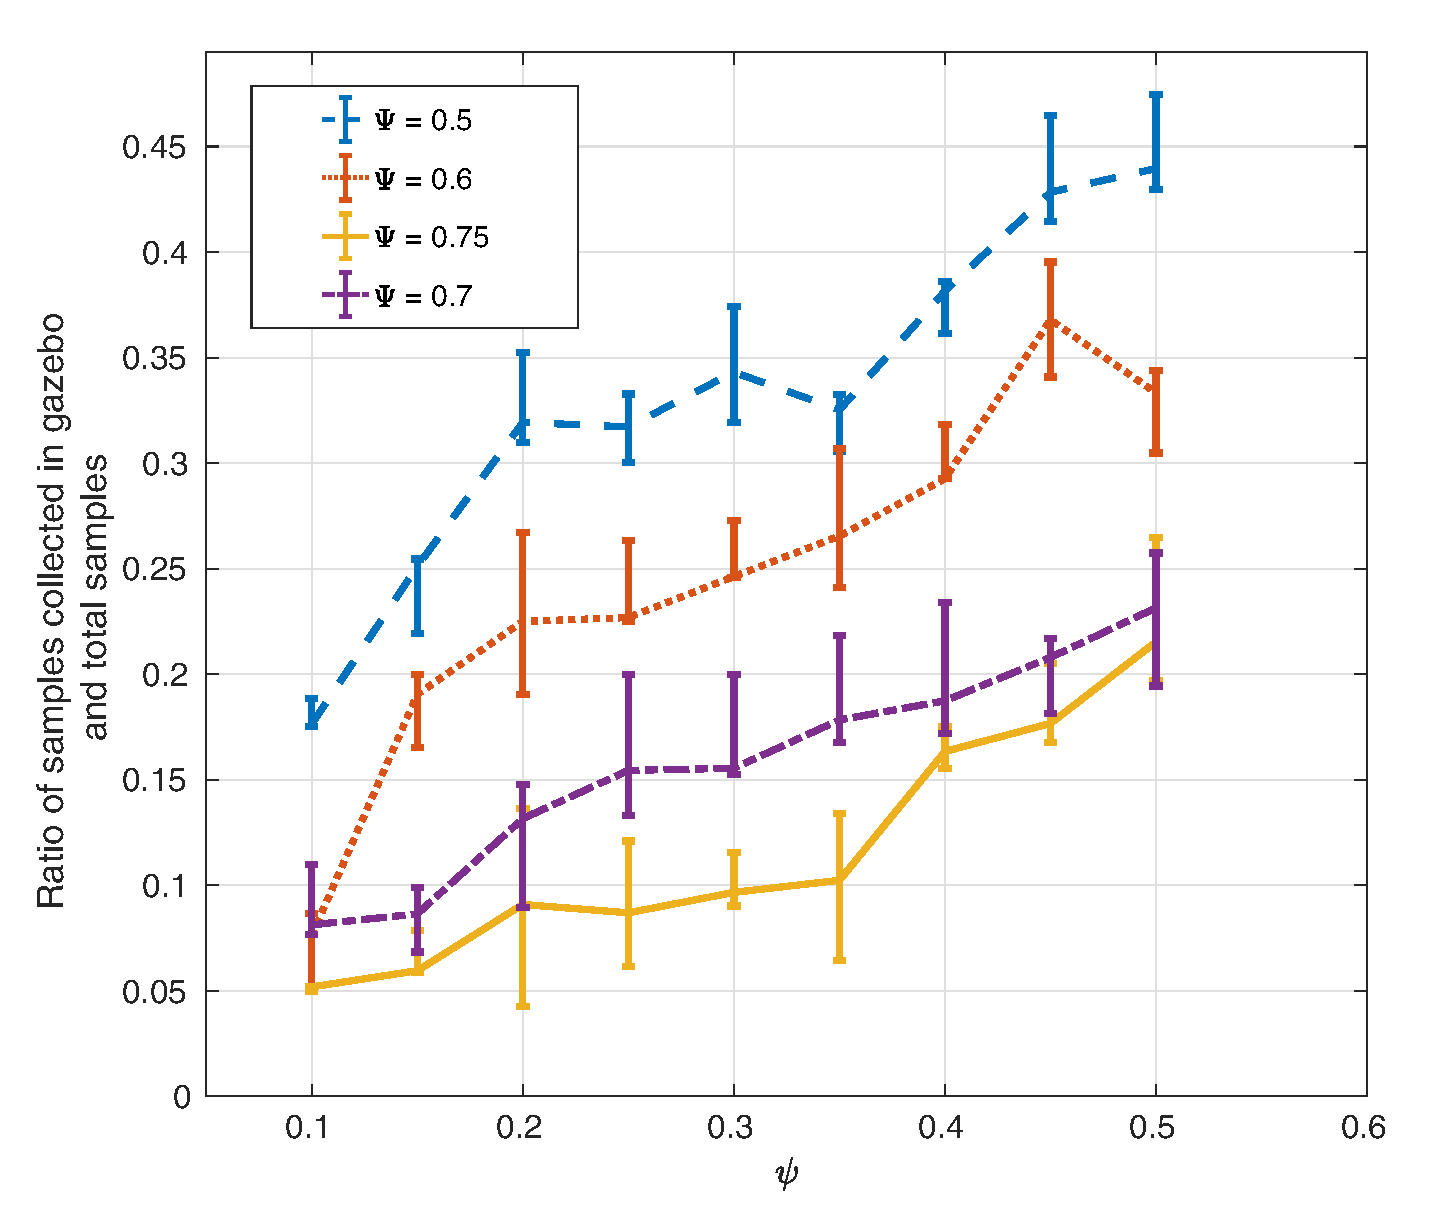
\includegraphics[width=8cm]{thre.eps} 
	\caption{Ratio of samples gathered in second simulator vs. total samples gathered as we change the threshold or confidence parameters of the two simulators.}
   \label{fig:threshold}
\end{figure}

\subsection{Comparison with R-max MFRL}
Figure \ref{fig:value_function} shows the comparison between performance of GP-MFRL algorithm with the existing MFRL algorithm \cite{cutler2014reinforcement}, GP-MFRL algorithm only in the highest fidelity simulator and Rmax algorithm running only in the highest fidelity simulator. The experiments are performed in the environment same as the one used in Figure \ref{fig:heatmap_four_walls_complex}. As expected, the GP-MFRL algorithm performs better than the existing MFRL algorithm, \cite{cutler2014reinforcement}.
\begin{figure}[htp]
	\centering 
    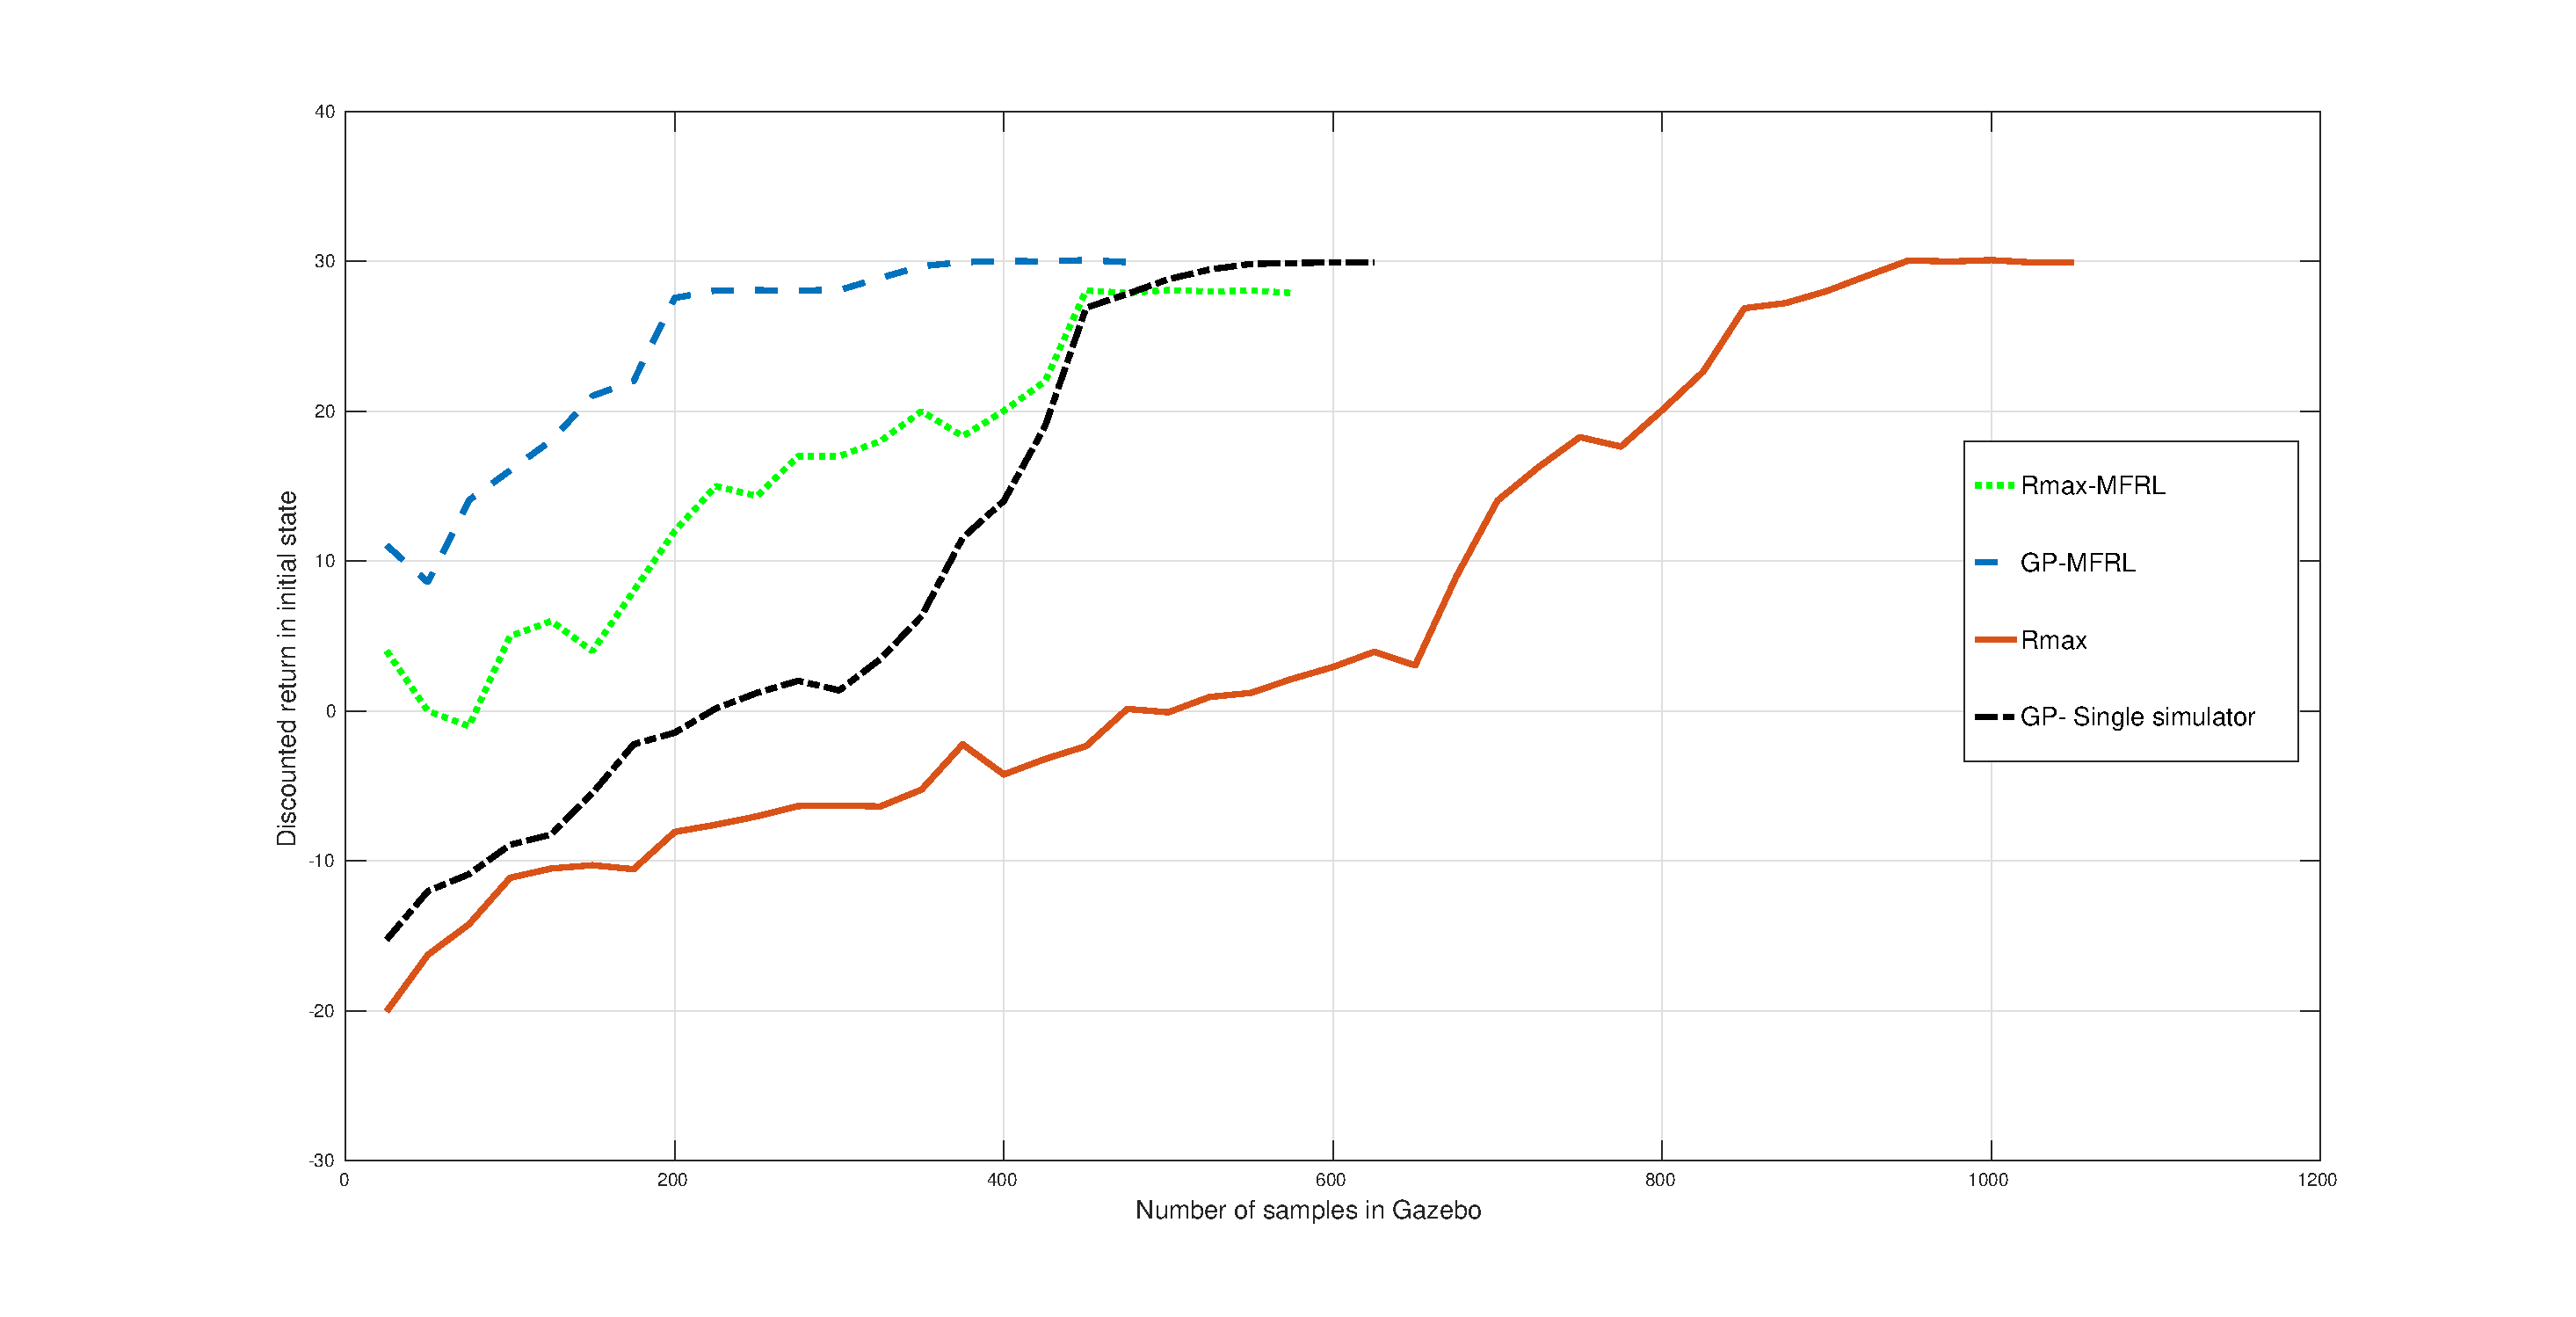
\includegraphics[width=8cm]{reward.eps}
	\caption{ Discounted return in the start state Vs. the number of samples collected in the highest fidelity simulator.}
   \label{fig:value_function}
\end{figure}

\section{Conclusion}
The GP-MFRL algorithm provides a general RL technique that is particularly suited for robotics. An extension to the existing work would be implementing the GP-MFRL algorithm on an actual quadrotor as the highest-fidelity simulator to demonstrate the utility of GP-MFRL. In this thesis, it is shown empirically that, GP-MFRL finds optimal policies using fewer samples than MFRL algorithm. 


\chapter{Bridge Inspection}
\section{Background}
When it comes to inspecting bridges, UAVs are often considered as harbingers, a truly disruptive technology capable of giving engineers eyes in the hardest to reach places, without the need for expensive access vehicles or potentially dangerous rigging or ladders or harnesses. A recent paper  \cite{morgenthal2014quality} discusses the application of UAVs for visual inspection and damage detection of civil structures. The quality of such pictures and videos taken by the UAV strongly depends on various factors viz. lighting conditions, distance from the structure, vehicle motion influenced by environmental effects etc. It is very important for the UAVs to be equipped with sophisticated control algorithms and sensors to be able to provide reliable data which can be conclusively used for inspection and analysis of damage.

\subsection{Conventional Inspection of Bridges}
Figure \ref{fig:bridge_inspection} shows typical inspection units like under-bridge units or truck cranes. Inspection units are in most cases expensive custom products. Often, specially trained staff, like industrial climbers, can get access to special parts of the structure but they can rarely evaluate what influences detected damages have on these structures. Therefore, they can only take Photos or Videos of the concerned part of the structure, which must be analyzed by civil engineers off-line.\par It is often dangerous to use such large truck cranes. Figure \ref{bridge_fail} shows an unfortunate incidence where the inspection truck has tipped over causing a life threating situation for the people involved.\par
 
\begin{figure}[htp]
	\centering 
    \subfigure[Truck Crane]{\includegraphics[width=6cm,height=4cm]{truck_crane.jpg}}
    \subfigure[Under Bridge Inspection unit]{\includegraphics[width=6cm,height=4cm]{under_bridge.jpg}}
	\caption{Conventional inspection units for Bridge Inspection: (left,Bridge Inspection platform with a truck crane) , A-30 Hi-Rail Under Bridge Units(right,N.E. Bridge Contractors Inc.)}
   \label{fig:bridge_inspection}
\end{figure}

\begin{figure}[htp]
	\centering 
    \includegraphics[width=8cm]{tip.jpg}
	\caption{Bridgeriggers' Aspen A-75 under-bridge inspection crane overturns on Sakonnet River Bridge in Rhode Island; August 30, 2016}
   \label{fig:bridge_fail}
\end{figure}

\subsection{UAVs in Bridge Inspection}

UAVs often have following advantages in comparison to the conventional bridge-inspection methods.
\begin{itemize}
\item  UAVs only need an operator on the ground for controlling the flight and the
camera. A more advanced scenario includes \textit{autonomous} UAVs navigating around the structures while collecting the required data such as pictures, videos etc. {\color{red} reference to a later section where we talk about challenges of navigating around such structures.}
\item UAVs can be used in high-risk situations without endangering human lives. Situations like \ref{fig:bridge_fail} could be avoided to a certain extent.
\item UAVs are capable of fast real time data acquisition and the storage of all the relevant flight data.
\item Overall, they often turn out to be lower in costs compared to the large custom inspection units.
\end{itemize}

As they say \textit{Every good thing comes with a price}, UAVs are no different. Despite the obvious advantages, UAVs have some essential limitations. 
\begin{itemize}
\item  Due to the small payload capacity of the UAVs, only small format and light digital compact cameras can be used for visual inspection. 
\item The smaller payload also affects the battery size leading to shorter flight times. 
\item Due to unexpected flight situations or due to unreliable GPS-signal strength, a change from the autonomous flight mode into a manual mode is required which demands a skillful pilot to override the control.
\item  Currently, UAVs are not equipped with effective collision avoidance systems. 
\end{itemize}

\section{Present Work}
We performed a few experiments in order to analyze the limitations and challenges of performing autonomous navigation of UAVs around bridges. We performed several manual flights of a UAV on the Smart Road Bridge (the tallest state-maintained bridge in Virginia). The goal of the experiment was to capture visuals of the inside as well as the outside of the bridge for analysis of the structure and to analyze challenges in order to improve the system for fully autonomous flights.

\subsection{The System Setup}
DJI model F450 \cite{dji_frame} was used as shown in the figure \ref{fig:dji_frame}. The UAV is equipped with sensors, controller and an on-board computer.

\begin{figure}[htp]
	\centering 
    \includegraphics[width=8cm]{uav-1.JPG}Init
	\caption{UAV used for the experiments}
   \label{fig:dji_frame}
\end{figure}
\todo{Add pictures and more information about the system}
\begin{itemize}
\item Camera: The camera used to capture the visuals was \cite{flea_camera}. The resolution of the images is $1600 \times 1200$ and can capture images upto $59$ FPS.
\item Intel NUC:
\item Pixhawk-Flight Controller:
\item LIDAR:
\item GPS: 
\end{itemize}

\subsection{Flights without GPS signal}
While the UAV is flying indoors or inside the bridge, it does not get a GPS signal for a better position estimate. Manual control is very difficult due to the smaller space and narrow pathways. In section \ref{gpq}, we discussed the advantages of effectively learning obstacle avoidance or wall-following as a skill using the on-board sensor data. It is very useful in these scenarios where the UAV needs to rely on it's on-board sensors to perform a particular task simultaneously trying to avoid obstacles or follow a wall. Figure \ref{fig:indoor_flight} indicates one such scenario where the UAV needs to take pictures inside the structures.
\begin{figure}[htp]
	\centering 
  	\subfigure{\includegraphics[width=8cm]{indoor_1.JPG}}
    \subfigure{\includegraphics[width=8cm]{indoor_2.jpeg}}
	\caption{Indoor flight of the UAV visually inspecting the structure}
   \label{fig:indoor_flight}
\end{figure}
Init
\subsection{Outdoor Inspection}
Figure \ref{fig:outdoor_flight}.
\begin{figure}[htp]
	\centering 
  	\subfigure{\includegraphics[width=8cm]{outdoor_1.JPG}}
    \subfigure{\includegraphics[width=8cm]{outdoor_2.JPG}}
	\caption{Outdoor flight of the UAV visually inspecting the structure}
   \label{fig:outdoor_flight}
\end{figure}

% Do tables like this:
\begin{comment}
 \begin{table}
 \caption{The Graduate School wants captions above the tables.}
\begin{center}
 \begin{tabular}{ccc}
 x & 1 & 2 \\ \hline
 1 & 1 & 2 \\
 2 & 2 & 4 \\ \hline
 \end{tabular}
\end{center}
 \end{table}
\end{comment}
%%%%%%%%%%%%%%%%%%%%%%%%%%%%%%%%

% If you are using BibTeX, uncomment the following:
\bibliography{refs}
\bibliographystyle{plain}
%
% Otherwise, uncomment the following:
% \chapter*{Bibliography}

% \appendix

% In LaTeX, each appendix is a "chapter"
% \chapter{Program Source}


\end{document}
